%        File: algosbcourse.tex
%     Created: mer. nov. 20 10:00  2013 C
% Last Change: mer. nov. 20 10:00  2013 C
%
\documentclass[]{beamer}
\usepackage{epigraph}
\setlength{\epigraphwidth}{\textwidth}
\newcommand*\elide{\textup{[\,\dots]}}
\usepackage{tikz}
\usepackage{pgfplots}
\usetikzlibrary{decorations,decorations.pathreplacing}
\usetikzlibrary{arrows,positioning,shapes}
\usetikzlibrary{calc}
% Plane partition
% Author: Jang Soo Kim
%\documentclass{minimal}
\usepackage{tikz}
%%%<
%\usepackage{verbatim}
%\usepackage[active,tightpage]{preview}
%\PreviewEnvironment{tikzpicture}
%\setlength\PreviewBorder{5pt}%
%%%>

%\begin{comment}
%:Title: Plane partition
%
%Illustration of a `plane partition`_.
%
%.. _plane partition: http://mathworld.wolfram.com/PlanePartition.html
%
%\end{comment}
% Three counters
\newcounter{x}
\newcounter{y}
\newcounter{z}

% The angles of x,y,z-axes
\newcommand\xaxis{210}
\newcommand\yaxis{-30}
\newcommand\zaxis{90}

% The top side of a cube
\newcommand\topside[3]{
  \fill[fill=yellow!30, draw=black,shift={(\xaxis:#1)},shift={(\yaxis:#2)},
  shift={(\zaxis:#3)}] (0,0) -- (30:1) -- (0,1) --(150:1)--(0,0);
}

% The left side of a cube
\newcommand\leftside[3]{
  \fill[fill=red!30, draw=black,shift={(\xaxis:#1)},shift={(\yaxis:#2)},
  shift={(\zaxis:#3)}] (0,0) -- (0,-1) -- (210:1) --(150:1)--(0,0);
}

% The right side of a cube
\newcommand\rightside[3]{
  \fill[fill=blue!30, draw=black,shift={(\xaxis:#1)},shift={(\yaxis:#2)},
  shift={(\zaxis:#3)}] (0,0) -- (30:1) -- (-30:1) --(0,-1)--(0,0);
}

% The cube 
\newcommand\cube[3]{
  \topside{#1}{#2}{#3} \leftside{#1}{#2}{#3} \rightside{#1}{#2}{#3}
}

% Definition of \planepartition
% To draw the following plane partition, just write \planepartition{ {a, b, c}, {d,e} }.
%  a b c
%  d e

\newcommand\planepartition[1]{
 \setcounter{x}{-1}
  \foreach \a in {#1} {
    \addtocounter{x}{1}
    \setcounter{y}{-1}
    \foreach \b in \a {
      \addtocounter{y}{1}
      \setcounter{z}{-1}
      \foreach \c in {1,...,\b} {
        \addtocounter{z}{1}
        \cube{\value{x}}{\value{y}}{\value{z}}
      }
    }
  }
}

%\begin{document} 
%
%\begin{tikzpicture}
%\planepartition{{5,3,2,2},{4,2,2,1},{2,1},{1}}
%\end{tikzpicture}
%
%\end{document} 

\AtBeginSection[]
{
 \begin{frame}<beamer>
 \frametitle{Plan}
 \tableofcontents[currentsection]
 \end{frame}
}
\title{Clustering protein conformations using SOM}
\author{Guillaume Bouvier}
\date{November 28, 2013}
\begin{document}
\frame{\titlepage}
\section{Introduction and theory}
\frame{
    \frametitle{What is a cluster?}
    \epigraph{\elide many authors \elide attempt to define just what a cluster is in terms of internal cohesion -- \emph{homogeneity} -- and external isolation -- \emph{separation}.}{Everitt, 2011}
    \begin{columns}
        \begin{column}{.5\textwidth}
            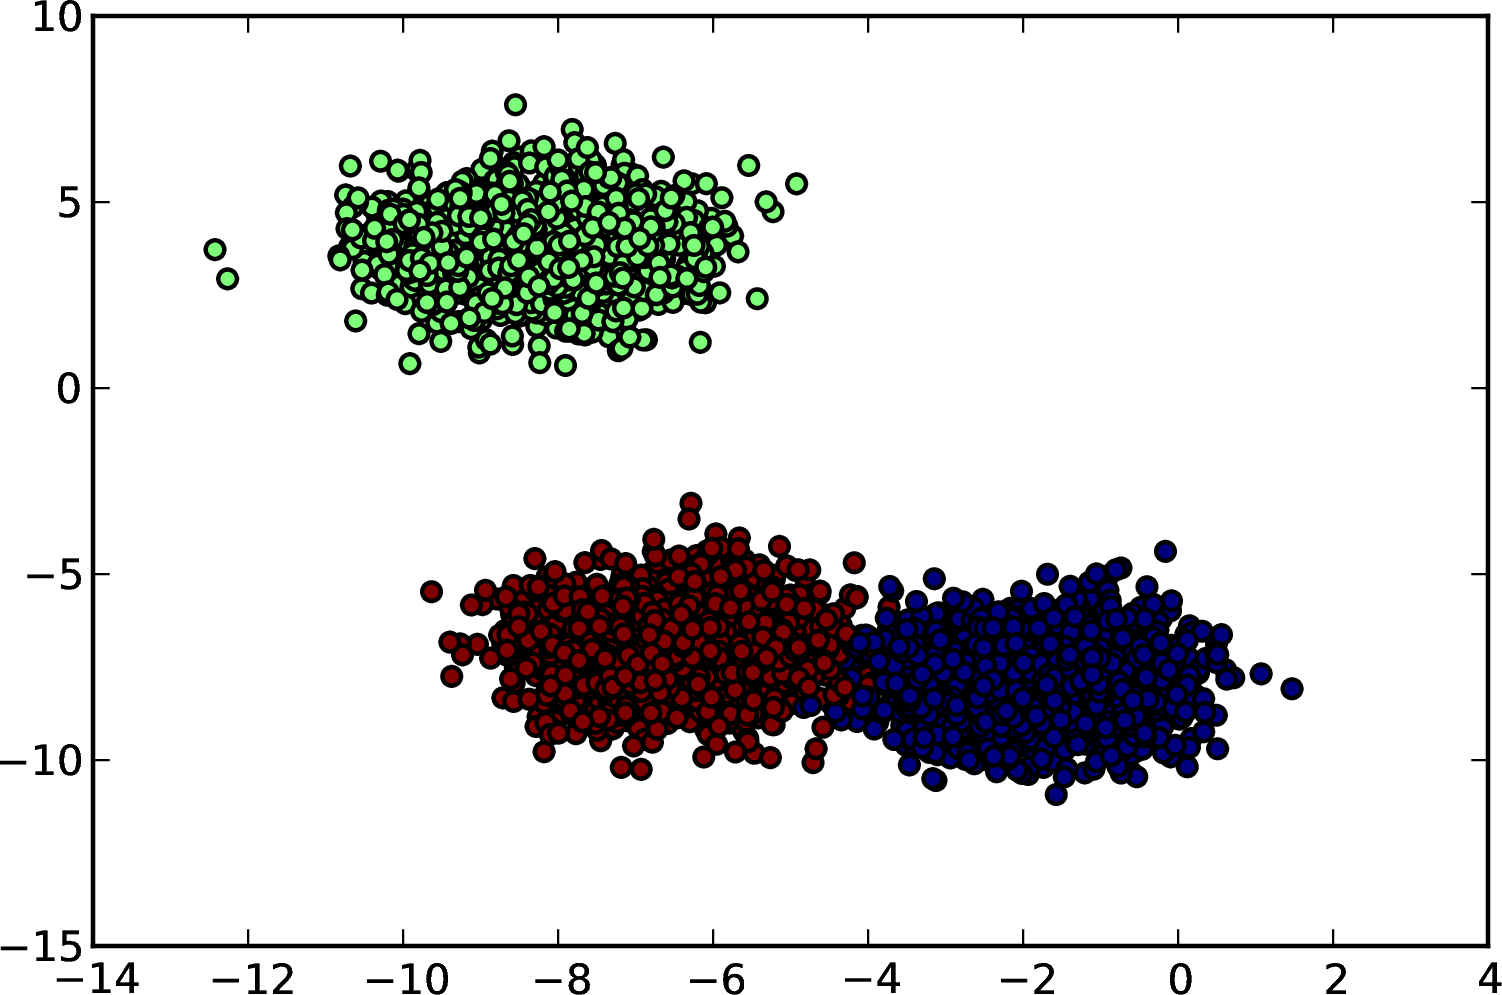
\includegraphics[width=\textwidth]{figures/dataset_blob.png}
        \end{column}
        \begin{column}{.5\textwidth}
            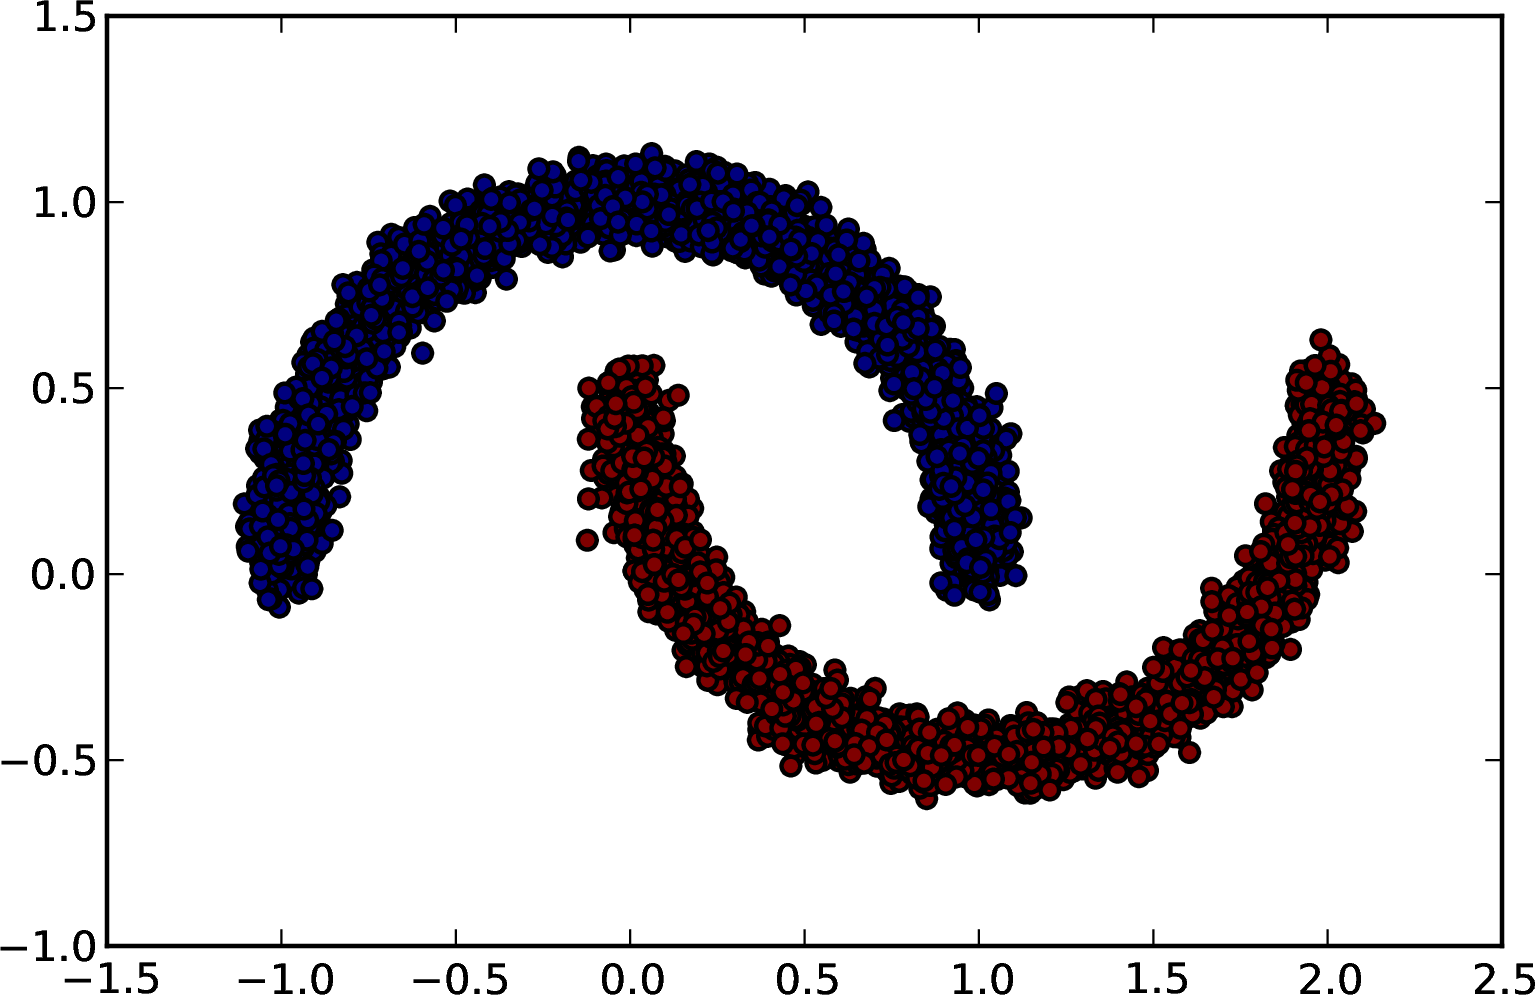
\includegraphics[width=\textwidth]{figures/dataset_moon.png}
        \end{column}
    \end{columns}

    Clusters with \textbf{internal cohesion} and/or \textbf{external isolation}.

}

\frame{
    \frametitle{What is a SOM?}
    \begin{itemize}
        \item SOM stand for \textbf{Self-Organizing Map} and was first described by the Finnish professor Teuvo Kohonen.
        \item A SOM is an \textbf{artificial neural network} that is trained using an \textbf{unsupervised learning} process.
        \item The \textbf{dimension of the SOM} ($X \times Y$) is chosen by the user (only 2D SOM will be aborded).
        \item Mathematically, a 2D-SOM is a \textbf{3D-matrix} of dimension ($X \times Y \times n$) with $n$ the dimension of the input space.
        \item A \textbf{neuron} is a cell characterized by its position $(i,j)$ in the ($X \times Y$) plane of the SOM. Its dimension is $n$.
    \end{itemize}
}

\frame{
    \frametitle{SOM architecture}
    \begin{columns}
        \begin{column}{.8\textwidth}
            \begin{center}
                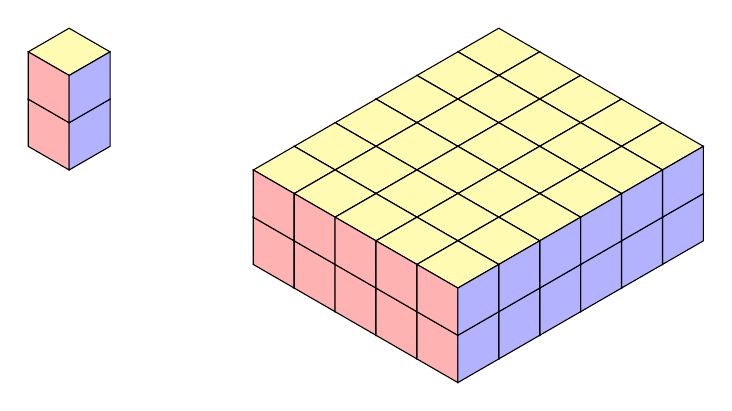
\begin{tikzpicture}[scale=0.6]
                    \begin{scope}
                        \planepartition{{2}}\vspace{0.25\textwidth}
                    \end{scope}
                    \begin{scope}[xshift=0.75\textwidth]
                        \planepartition{
                            {2,2,2,2,2},
                            {2,2,2,2,2},
                            {2,2,2,2,2},
                            {2,2,2,2,2},
                            {2,2,2,2,2},
                            {2,2,2,2,2},
                        }
                    \end{scope}
                \end{tikzpicture}
            \end{center}
        \end{column}
        \begin{column}{.2\textwidth}
            
\includegraphics[width=\textwidth]{figures/donut.png}

            A torus!
        \end{column}
    \end{columns}
    Example of an input vector of dimension $n=2$ and a SOM of dimension $5 \times 5$. The SOM is periodic: a torus.
}

\frame{
    \frametitle{Initialization of the SOM}
    The SOM is initialized randomly with an uniform distribution within the range of the input data.
    \begin{columns}
        \begin{column}{.6\textwidth}
            \begin{center}
                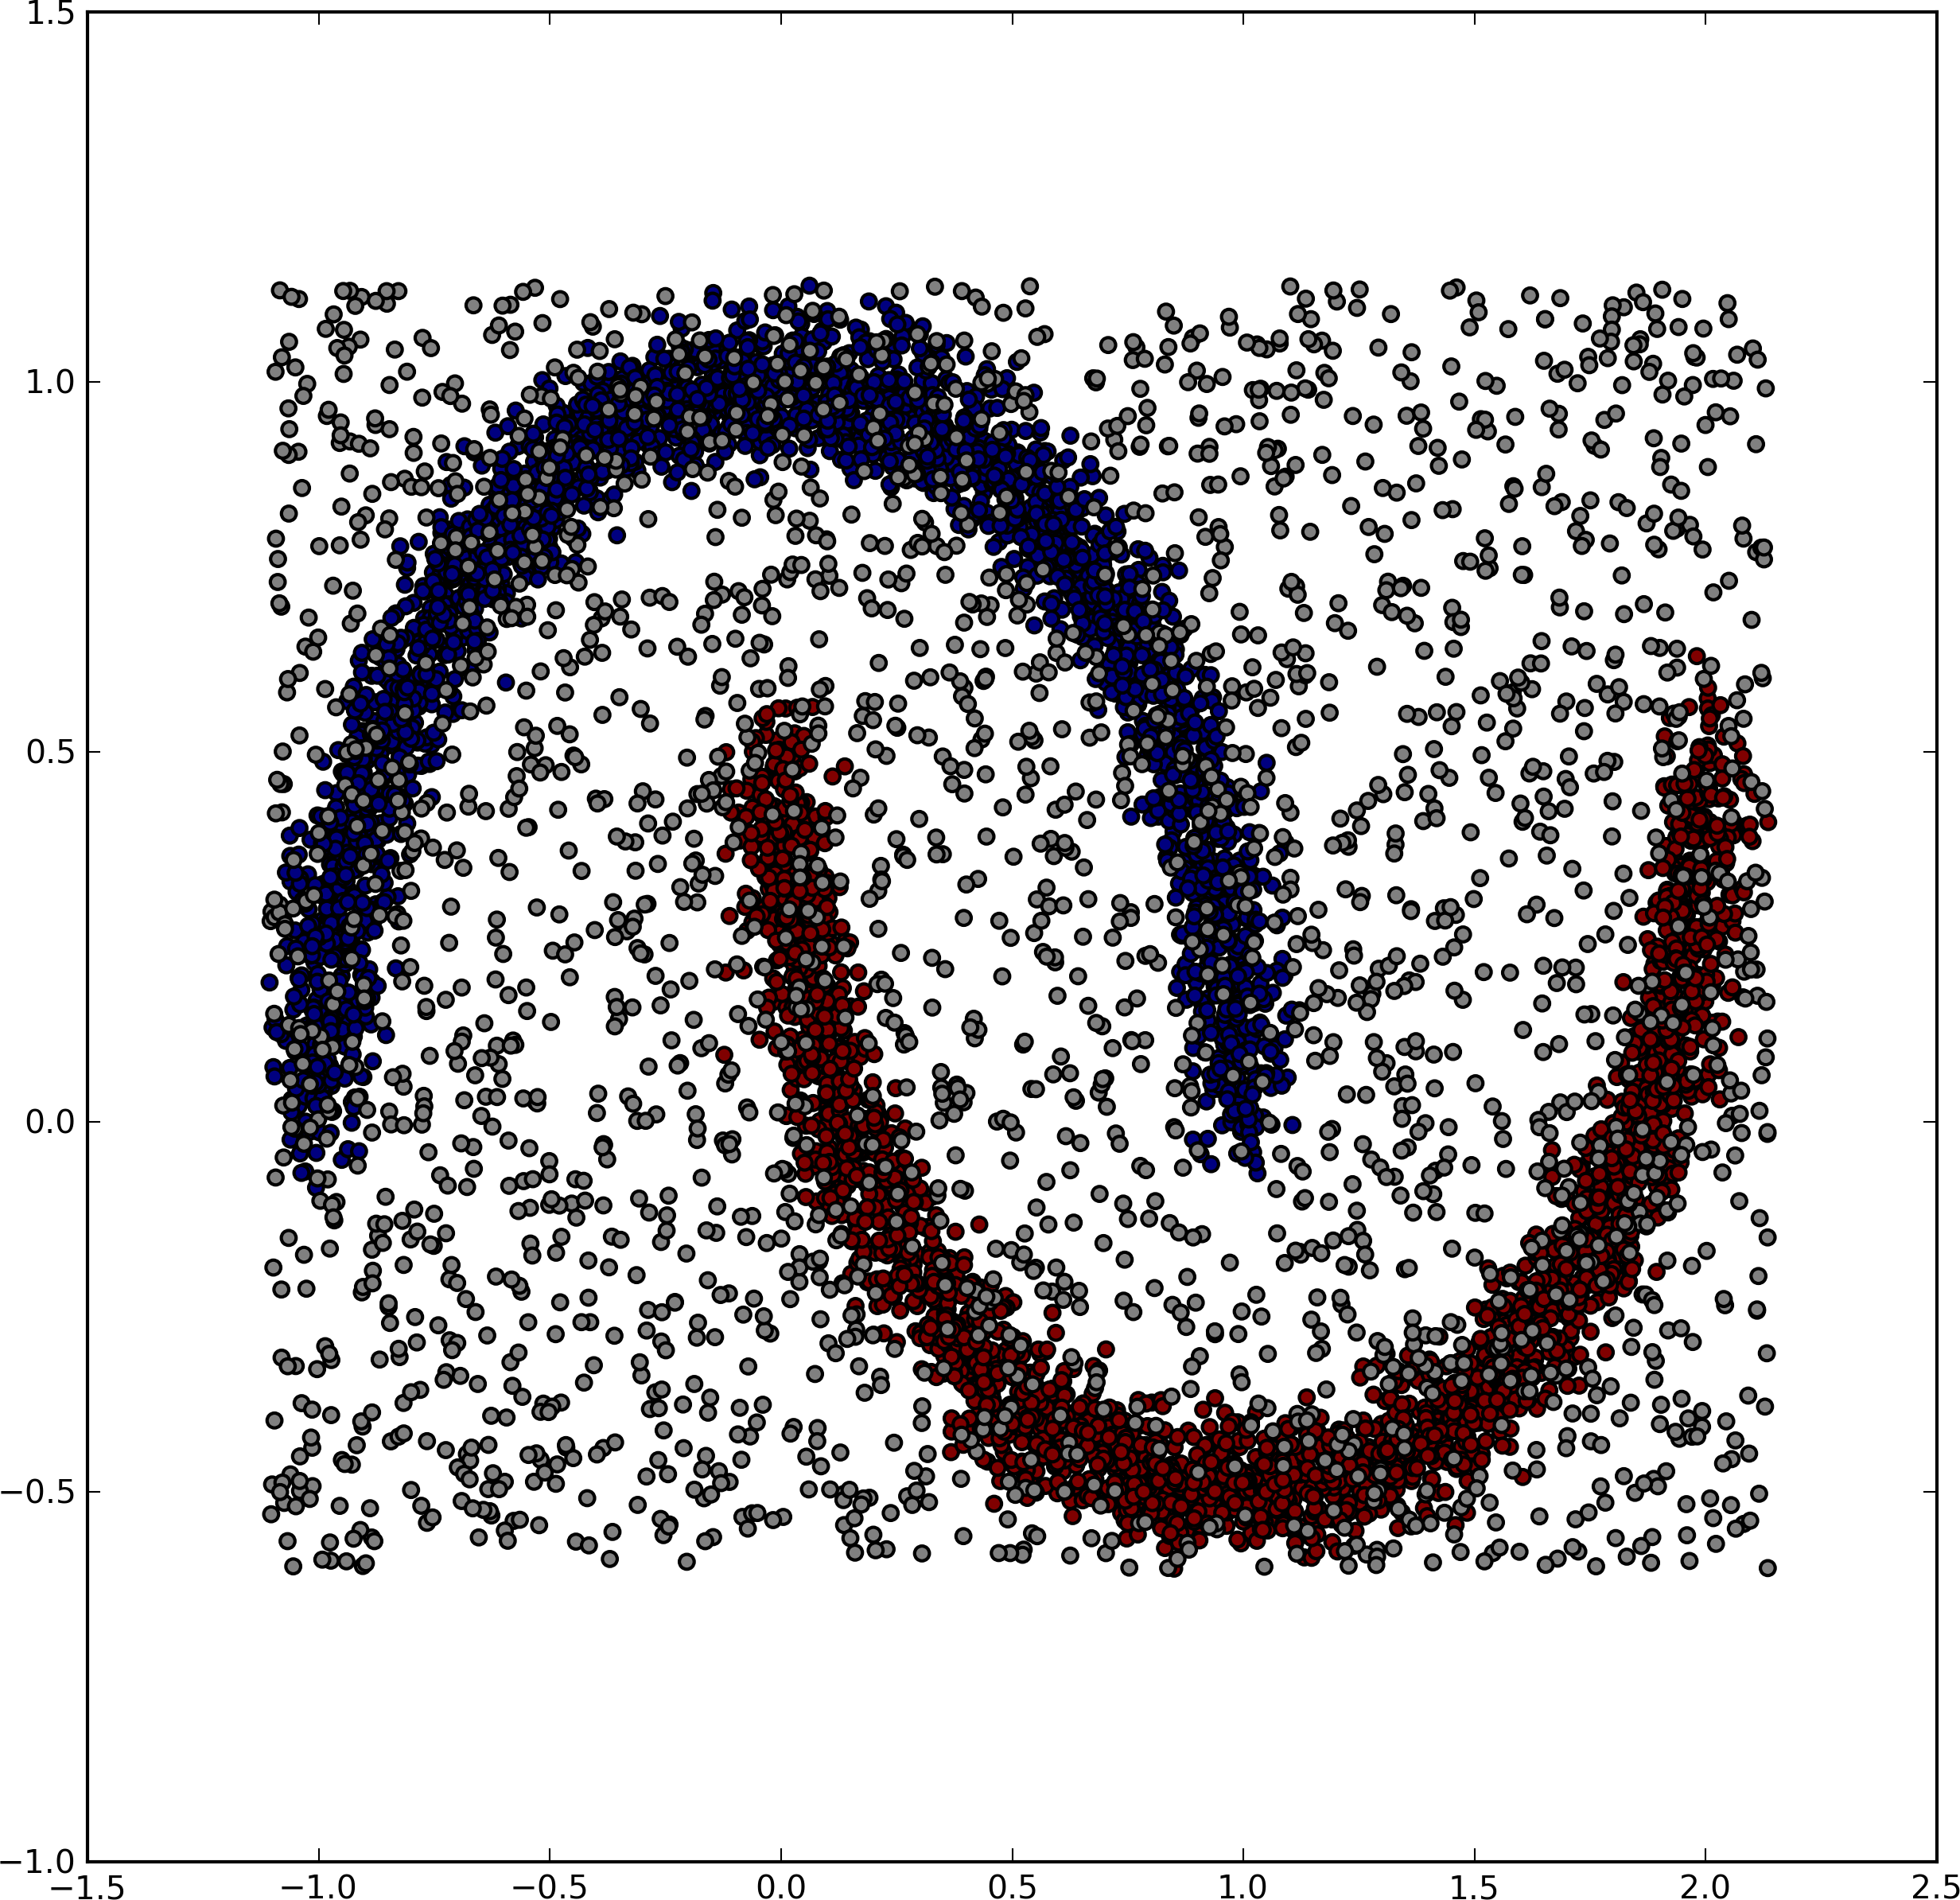
\includegraphics[width=\textwidth]{figures/sominit.png}
            \end{center}
        \end{column}
        \begin{column}{.4\textwidth}
            Example of SOM initialization on the moon dataset. 
            Take care to differentiate the \textbf{SOM space} which is a \textbf{2D lattice} of 2D vectors for this example and the \textbf{input space}, represented on the left.
        \end{column}
    \end{columns}
}

\frame{
    \frametitle{The algorithm}
    For each \textbf{iteration}
    \begin{itemize}
        \item we select randomly an input vector from the input space
        \item we compute the Euclidean distance between the input vector and each neuron of the map
        \item we select the neuron with the minimal distance, which is called the \textbf{Best Matching Unit} (BMU)
        \item we modified the map with the following formula:
    \end{itemize}
    \begin{exampleblock}{}
        \tikzstyle{every picture}+=[remember picture]
        \everymath{\displaystyle}
        \tikzstyle{na} = [baseline=-.5ex]
        \begin{itemize}
            \item Linear adjustment of the weights. \tikz[na] \node [coordinate] (adjustl) {};
            \item Neighborhood function: regulates the influence\\of the BMU $(\beta_{1},\beta{2})$ \tikz[na] \node [coordinate] (thetal) {}; on the neighboring neurons.
        \end{itemize}
        \begin{equation*}
            M(t+1) = M(t) + 
            \tikz[baseline]{ \node[fill=blue!20,anchor=base] (alpha) {$\alpha(t)$}; }
            \cdot
            \tikz[baseline]{ \node[fill=red!20,anchor=base] (theta) {$\Theta(t,\beta_{1},\beta{2})$}; }
            \cdot
            \tikz[baseline]{ \node[fill=green!20,anchor=base] (adjust) {$(V-\Omega_{ij}(t))_{1\leq i\leq X,1\leq j\leq Y}$}; }
        \end{equation*}
        \begin{itemize}
            \item Learning rate \tikz[na] \node [coordinate] (alphal) {};: weights the effect of the input vector during the training process.
        \end{itemize}
        \begin{tikzpicture}[overlay]
            \path[->] (adjustl) edge [out=45, in=40] (adjust);
            \path[->] (thetal) edge [out=-90,in=90] (theta);
            \path[->] (alphal) edge [out=90, in=-90] (alpha);
        \end{tikzpicture}
    \end{exampleblock}
}

\frame{
    \frametitle{The radius function}
    \begin{block}{Neighborhood function $\Theta$: the radius $\sigma$}
        \begin{equation*}
            \Theta(t,\beta_{1},\beta_{2})=\exp\left(-\frac{(i-\beta_{1})^{2}+(j-\beta_{2})^{2}}{2\sigma^{2}(t)}\right)
        \end{equation*}
        \begin{columns}
            \begin{column}{0.4\textwidth}
                $\sigma = 1.7$\\
                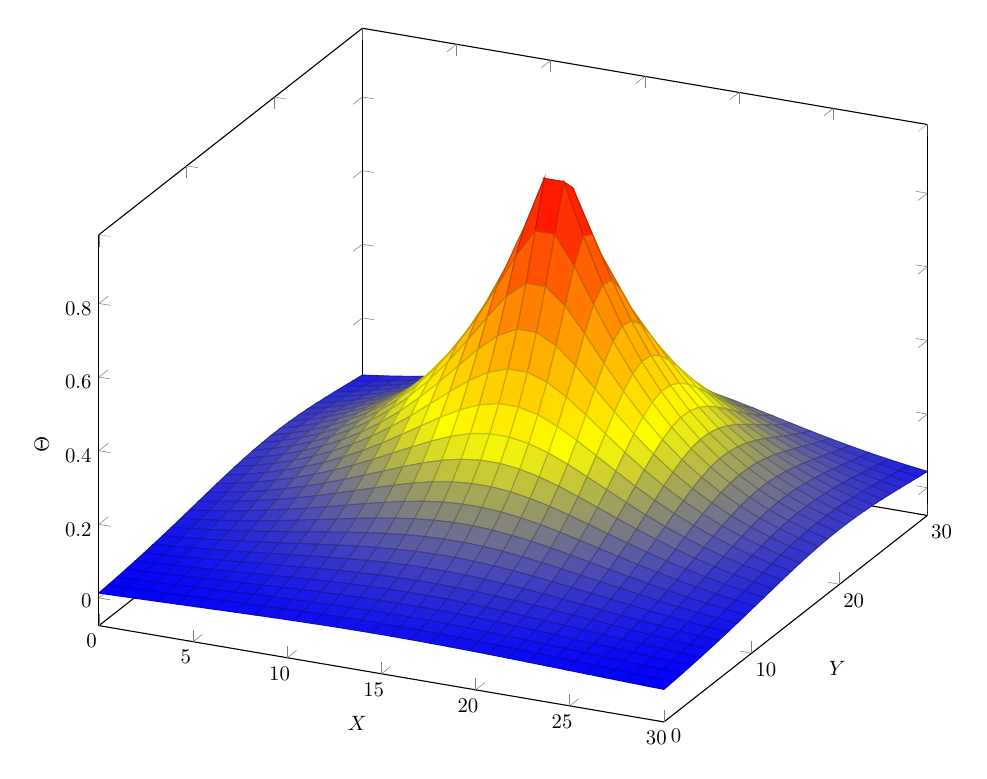
\begin{tikzpicture}[scale=1, every node/.style={scale=0.75}]
                    \pgfplotsset{width=\textwidth,compat=1.3}
                          \begin{axis}[xlabel=$X$, ylabel=$Y$,zlabel=$\Theta$]
                          \addplot3[surf,shader=faceted,domain=0:30,samples=30]
                              {exp( -1 * ( sqrt((x-15)^2+(y-20)^2)/(2*1.7^2) ) )};
                         \end{axis}
                \end{tikzpicture}
            \end{column}
            \begin{column}{0.4\textwidth}
                $\sigma=1$\\
                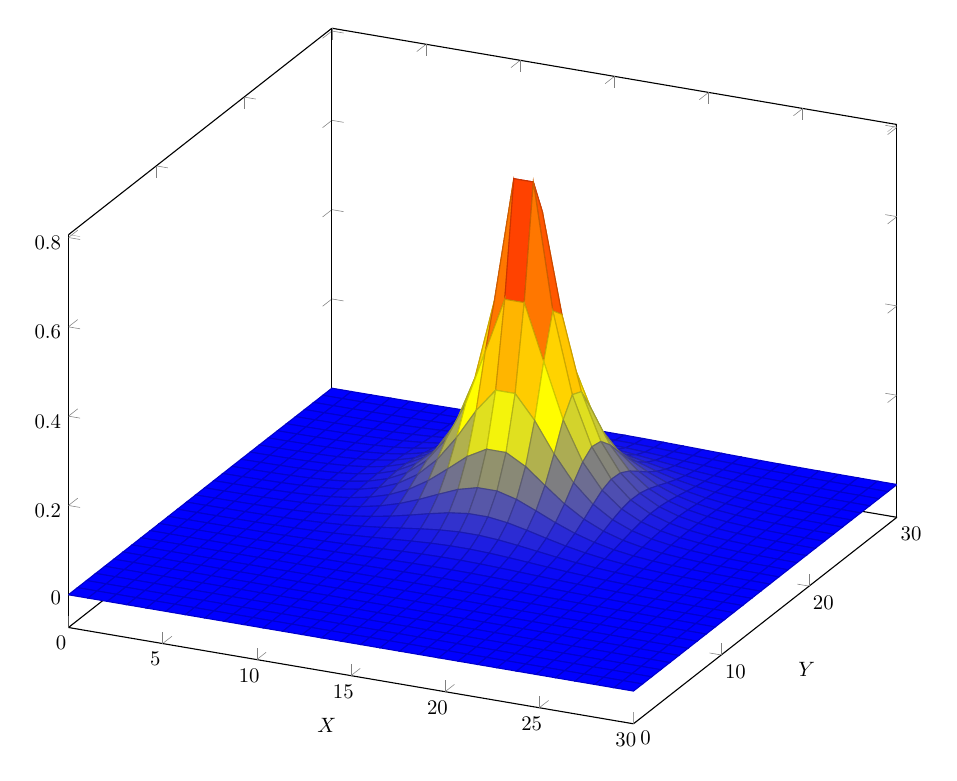
\begin{tikzpicture}[scale=1, every node/.style={scale=0.75}]
                    \pgfplotsset{width=\textwidth,compat=1.3}
                          \begin{axis}[xlabel=$X$, ylabel=$Y$]
                          \addplot3[surf,shader=faceted,domain=0:30,samples=30]
                              {exp( -1 * ( sqrt((x-15)^2+(y-20)^2)/(2*1^2) ) )};
                         \end{axis}
                \end{tikzpicture}
            \end{column}
        \end{columns}
        \begin{equation*}
            \sigma(t)=(\sigma(t_{i})-\sigma(t_{f}))\cdot\exp(-\frac{t}{\lambda})+\sigma(t_{f})
        \end{equation*}
    \end{block}
}

\frame{
    \frametitle{The learning rate}
    \begin{block}{Neighborhood function $\Theta$: the learning rate $\alpha$}
        \begin{equation*}
            \alpha(t)\cdot\Theta(t,\beta_{1},\beta_{2})
        \end{equation*}
        \begin{columns}
            \begin{column}{0.4\textwidth}
                $\sigma = 1.7$, $\alpha=0.5$\\
                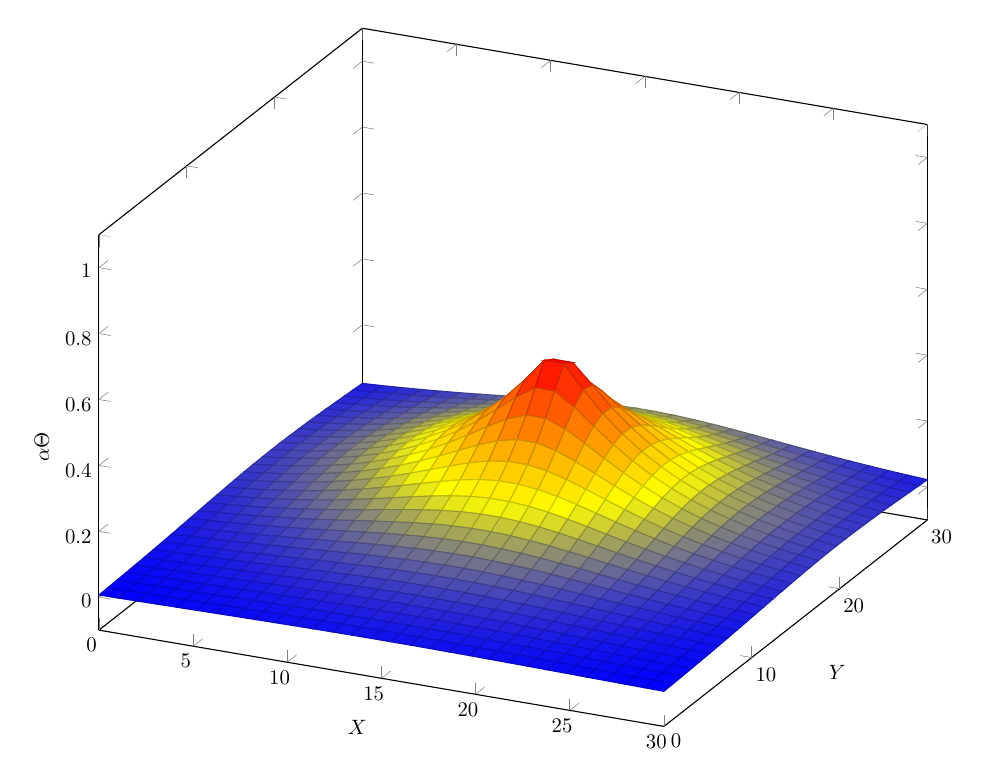
\begin{tikzpicture}[scale=1, every node/.style={scale=0.75}]
                    \pgfplotsset{width=\textwidth,compat=1.3}
                          \begin{axis}[xlabel=$X$, ylabel=$Y$,zlabel=$\alpha\Theta$]
                          \addplot3[surf,shader=faceted,domain=0:30, samples=30]
                              {0.5*(exp( -1 * ( sqrt((x-15)^2+(y-20)^2)/(2*1.7^2) ) ))};
                    \addplot3[color=black, mark=none] plot coordinates {(0,0,0) (0,0,1)};
                         \end{axis}
                \end{tikzpicture}
            \end{column}
            \begin{column}{0.4\textwidth}
                $\sigma=1$, $\alpha=0.25$\\
                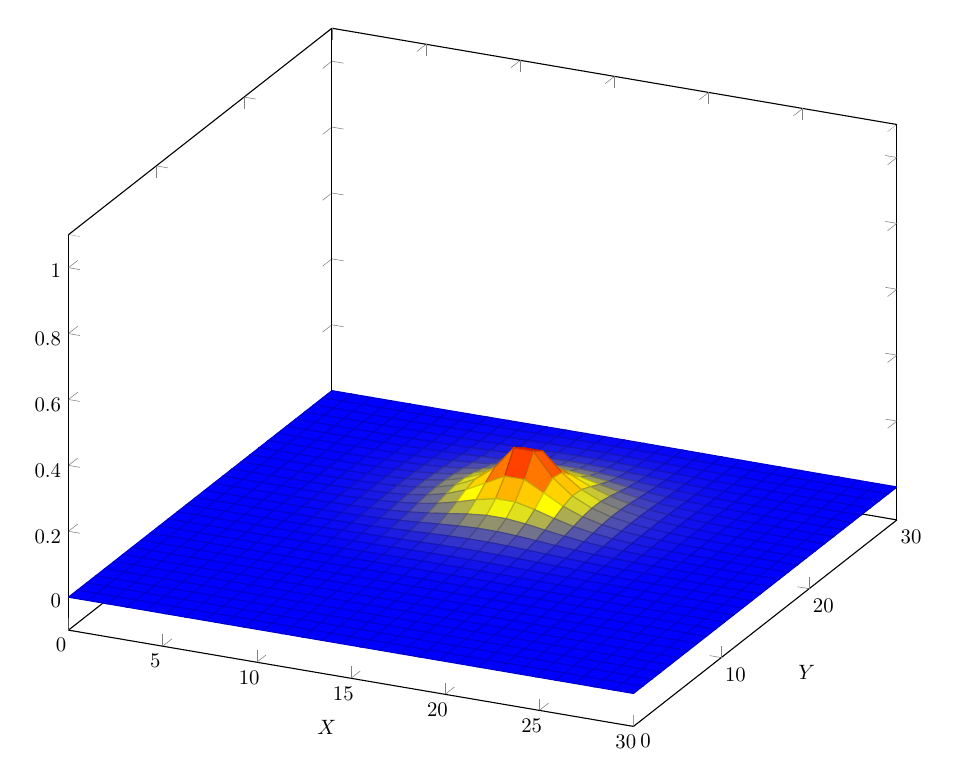
\begin{tikzpicture}[scale=1, every node/.style={scale=0.75}]
                    \pgfplotsset{width=\textwidth,compat=1.3}
                          \begin{axis}[xlabel=$X$, ylabel=$Y$]
                          \addplot3[surf,shader=faceted,domain=0:30, samples=30]
                              {0.25*(exp( -1 * ( sqrt((x-15)^2+(y-20)^2)/(2*1^2) ) ))};
                    \addplot3[color=black, mark=none] plot coordinates {(0,0,0) (0,0,1)};
                         \end{axis}
                \end{tikzpicture}
            \end{column}
        \end{columns}
        \begin{equation*}
        \alpha(t)=(\alpha(t_{i})-\alpha(t_{f}))\cdot\exp(-\frac{t}{\lambda})+\alpha(t_{f})
        \end{equation*}
    \end{block}
}

\frame{
    \frametitle{The trained SOM}
    \begin{columns}
        \begin{column}{.6\textwidth}
            \begin{center}
                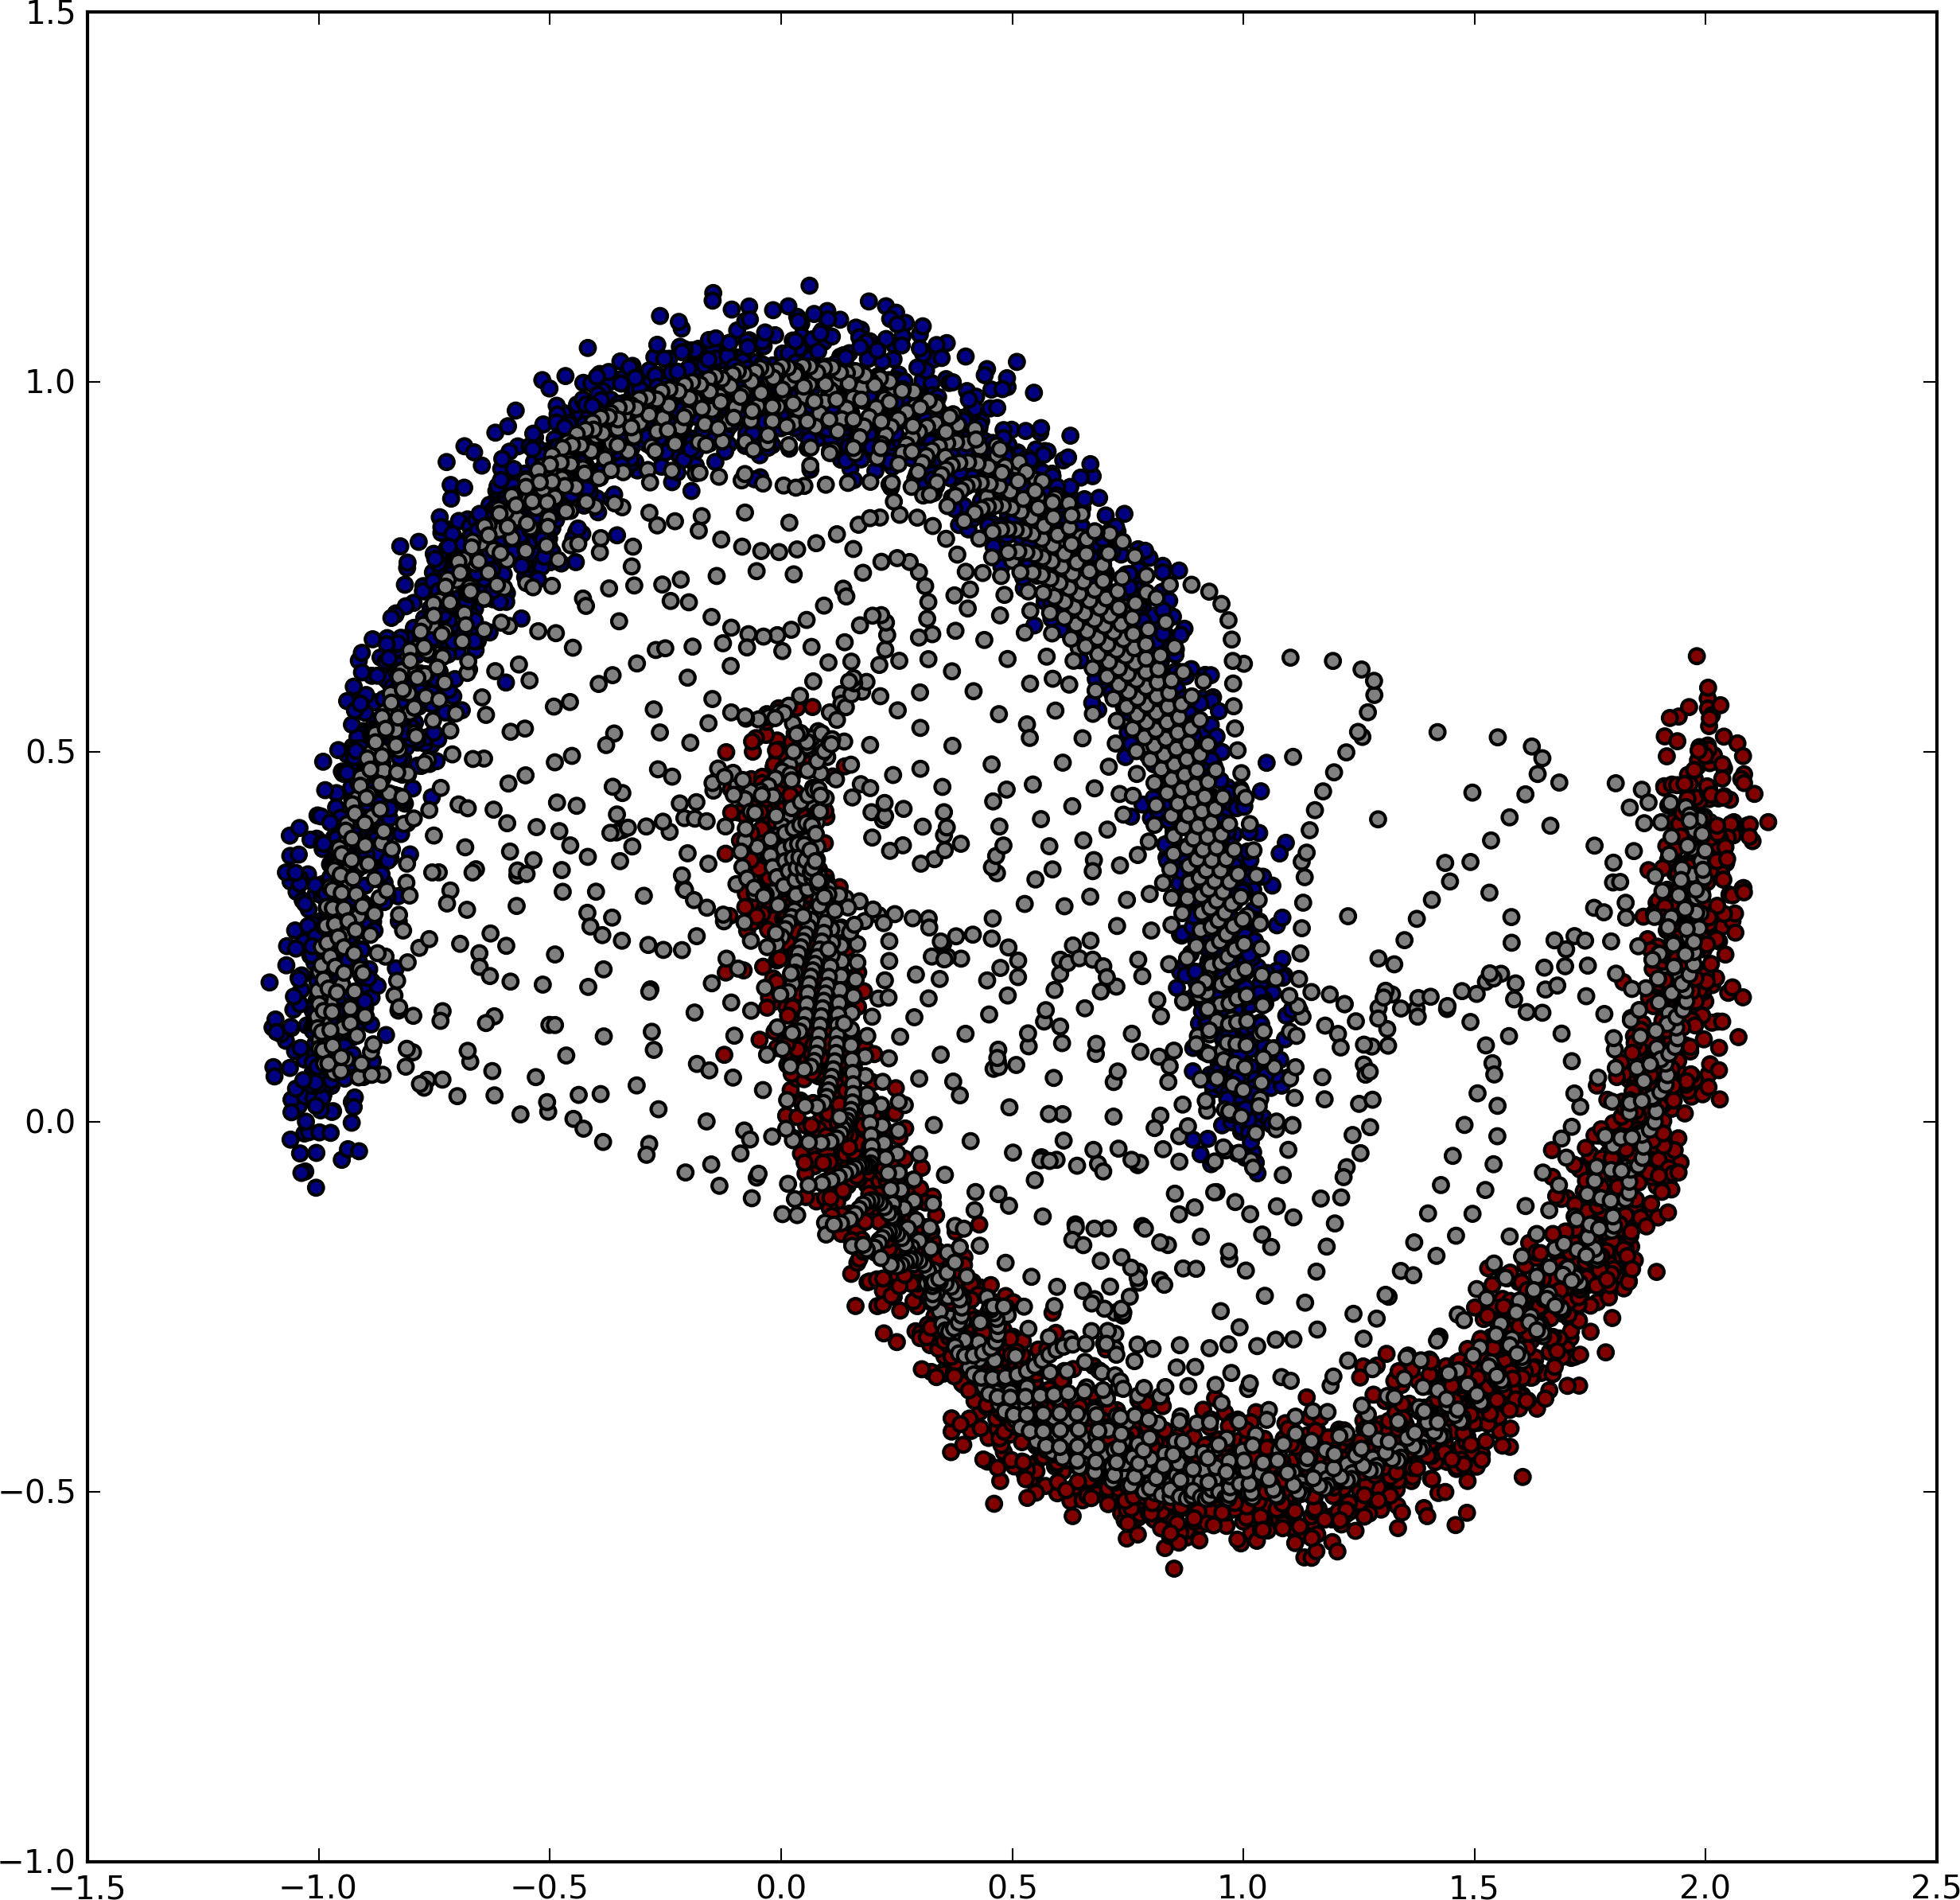
\includegraphics[width=\textwidth]{figures/somtrained.png}
            \end{center}
        \end{column}
        \begin{column}{.4\textwidth}
            Example of trained SOM with the moon dataset.
            The neurons are represented in the input space.
        \end{column}
    \end{columns}
}

\begin{frame}
    \frametitle{SOM parameters}
    \begin{description}
        \item[Map size] A map size \textbf{$50 \times 50$} is convenient to visualize the U-matrix and large enough to cluster large dataset.
        \item[Number of iterations] Splited in \textbf{two phases}. The number of iterations is equal to the number of input data for the first phase and twice this number for the second phase.
        \item[Learning rate] Starting from \textbf{0.5} and ending to \textbf{0.25} for the first phase and starting from \textbf{0.25} and ending to \textbf{0.0} for the second phase.
        \item[Radius] Starting from \textbf{6.25} and ending to \textbf{3.0} for the first phase and starting from \textbf{4.0} and ending to \textbf{1.0} for the second phase.
    \end{description}
\end{frame}

\frame{
    \frametitle{How to visualize the SOM space?}
    \begin{columns}
        \begin{column}{.5\textwidth}
            \begin{center}
                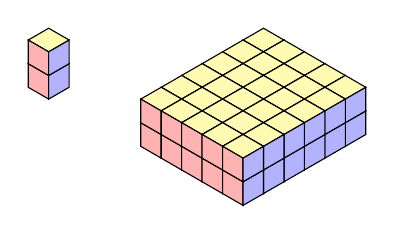
\begin{tikzpicture}[scale=0.3]
                    \begin{scope}
                        \planepartition{{2}}\vspace{0.25\textwidth}
                    \end{scope}
                    \begin{scope}[xshift=0.75\textwidth]
                        \planepartition{
                            {2,2,2,2,2},
                            {2,2,2,2,2},
                            {2,2,2,2,2},
                            {2,2,2,2,2},
                            {2,2,2,2,2},
                            {2,2,2,2,2},
                        }
                    \end{scope}
                \end{tikzpicture}
            \end{center}
        \end{column}
        \begin{column}{.65\textwidth}
            The U-matrix (Unified distance matrix) is the mean euclidean distance of each neuron with their eight neighbors.
            \begin{equation*}
                U = \frac{1}{8}\sum_{\mu in N(\nu)}d(\nu,\mu)
            \end{equation*}
            It gives the topology of the map.
            It allows the identification of ``natural`` clusters in the map.
        \end{column}
    \end{columns}
}

\frame{
    \frametitle{The U-matrix}
    \begin{columns}
        \begin{column}{.5\textwidth}
            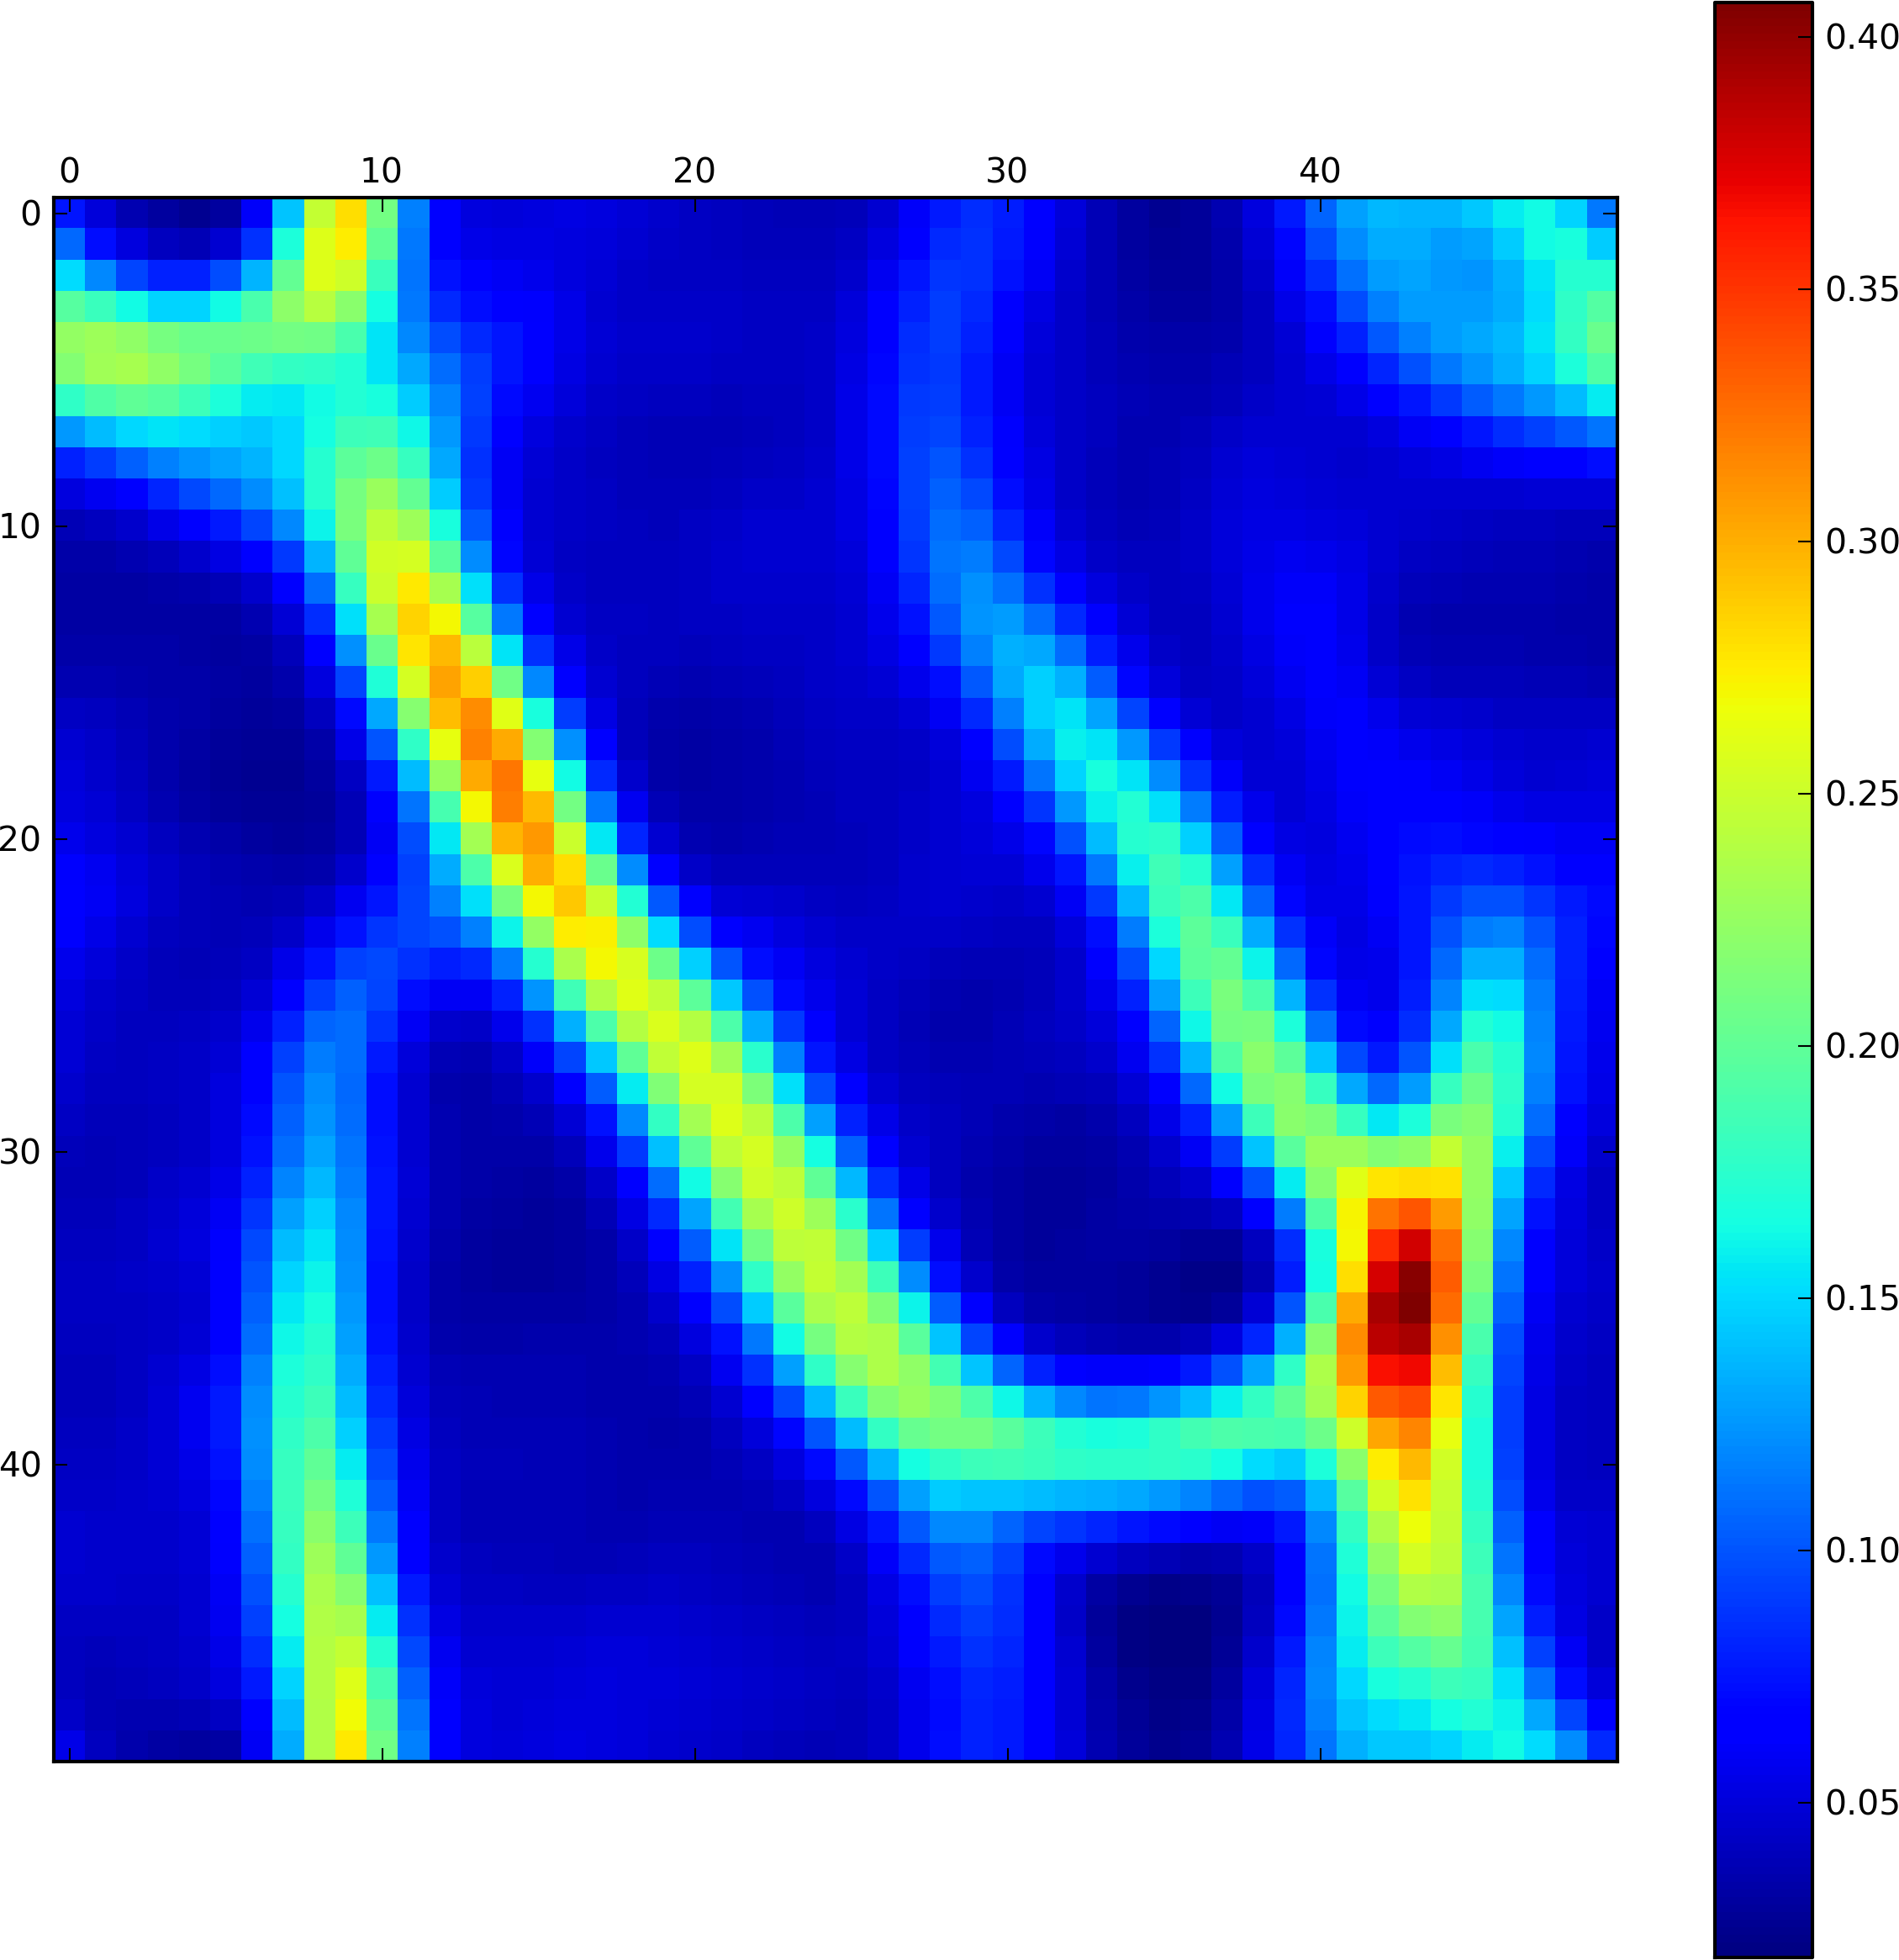
\includegraphics[width=\textwidth]{figures/umatrixmoon.png}
        \end{column}
        \begin{column}{.5\textwidth}
            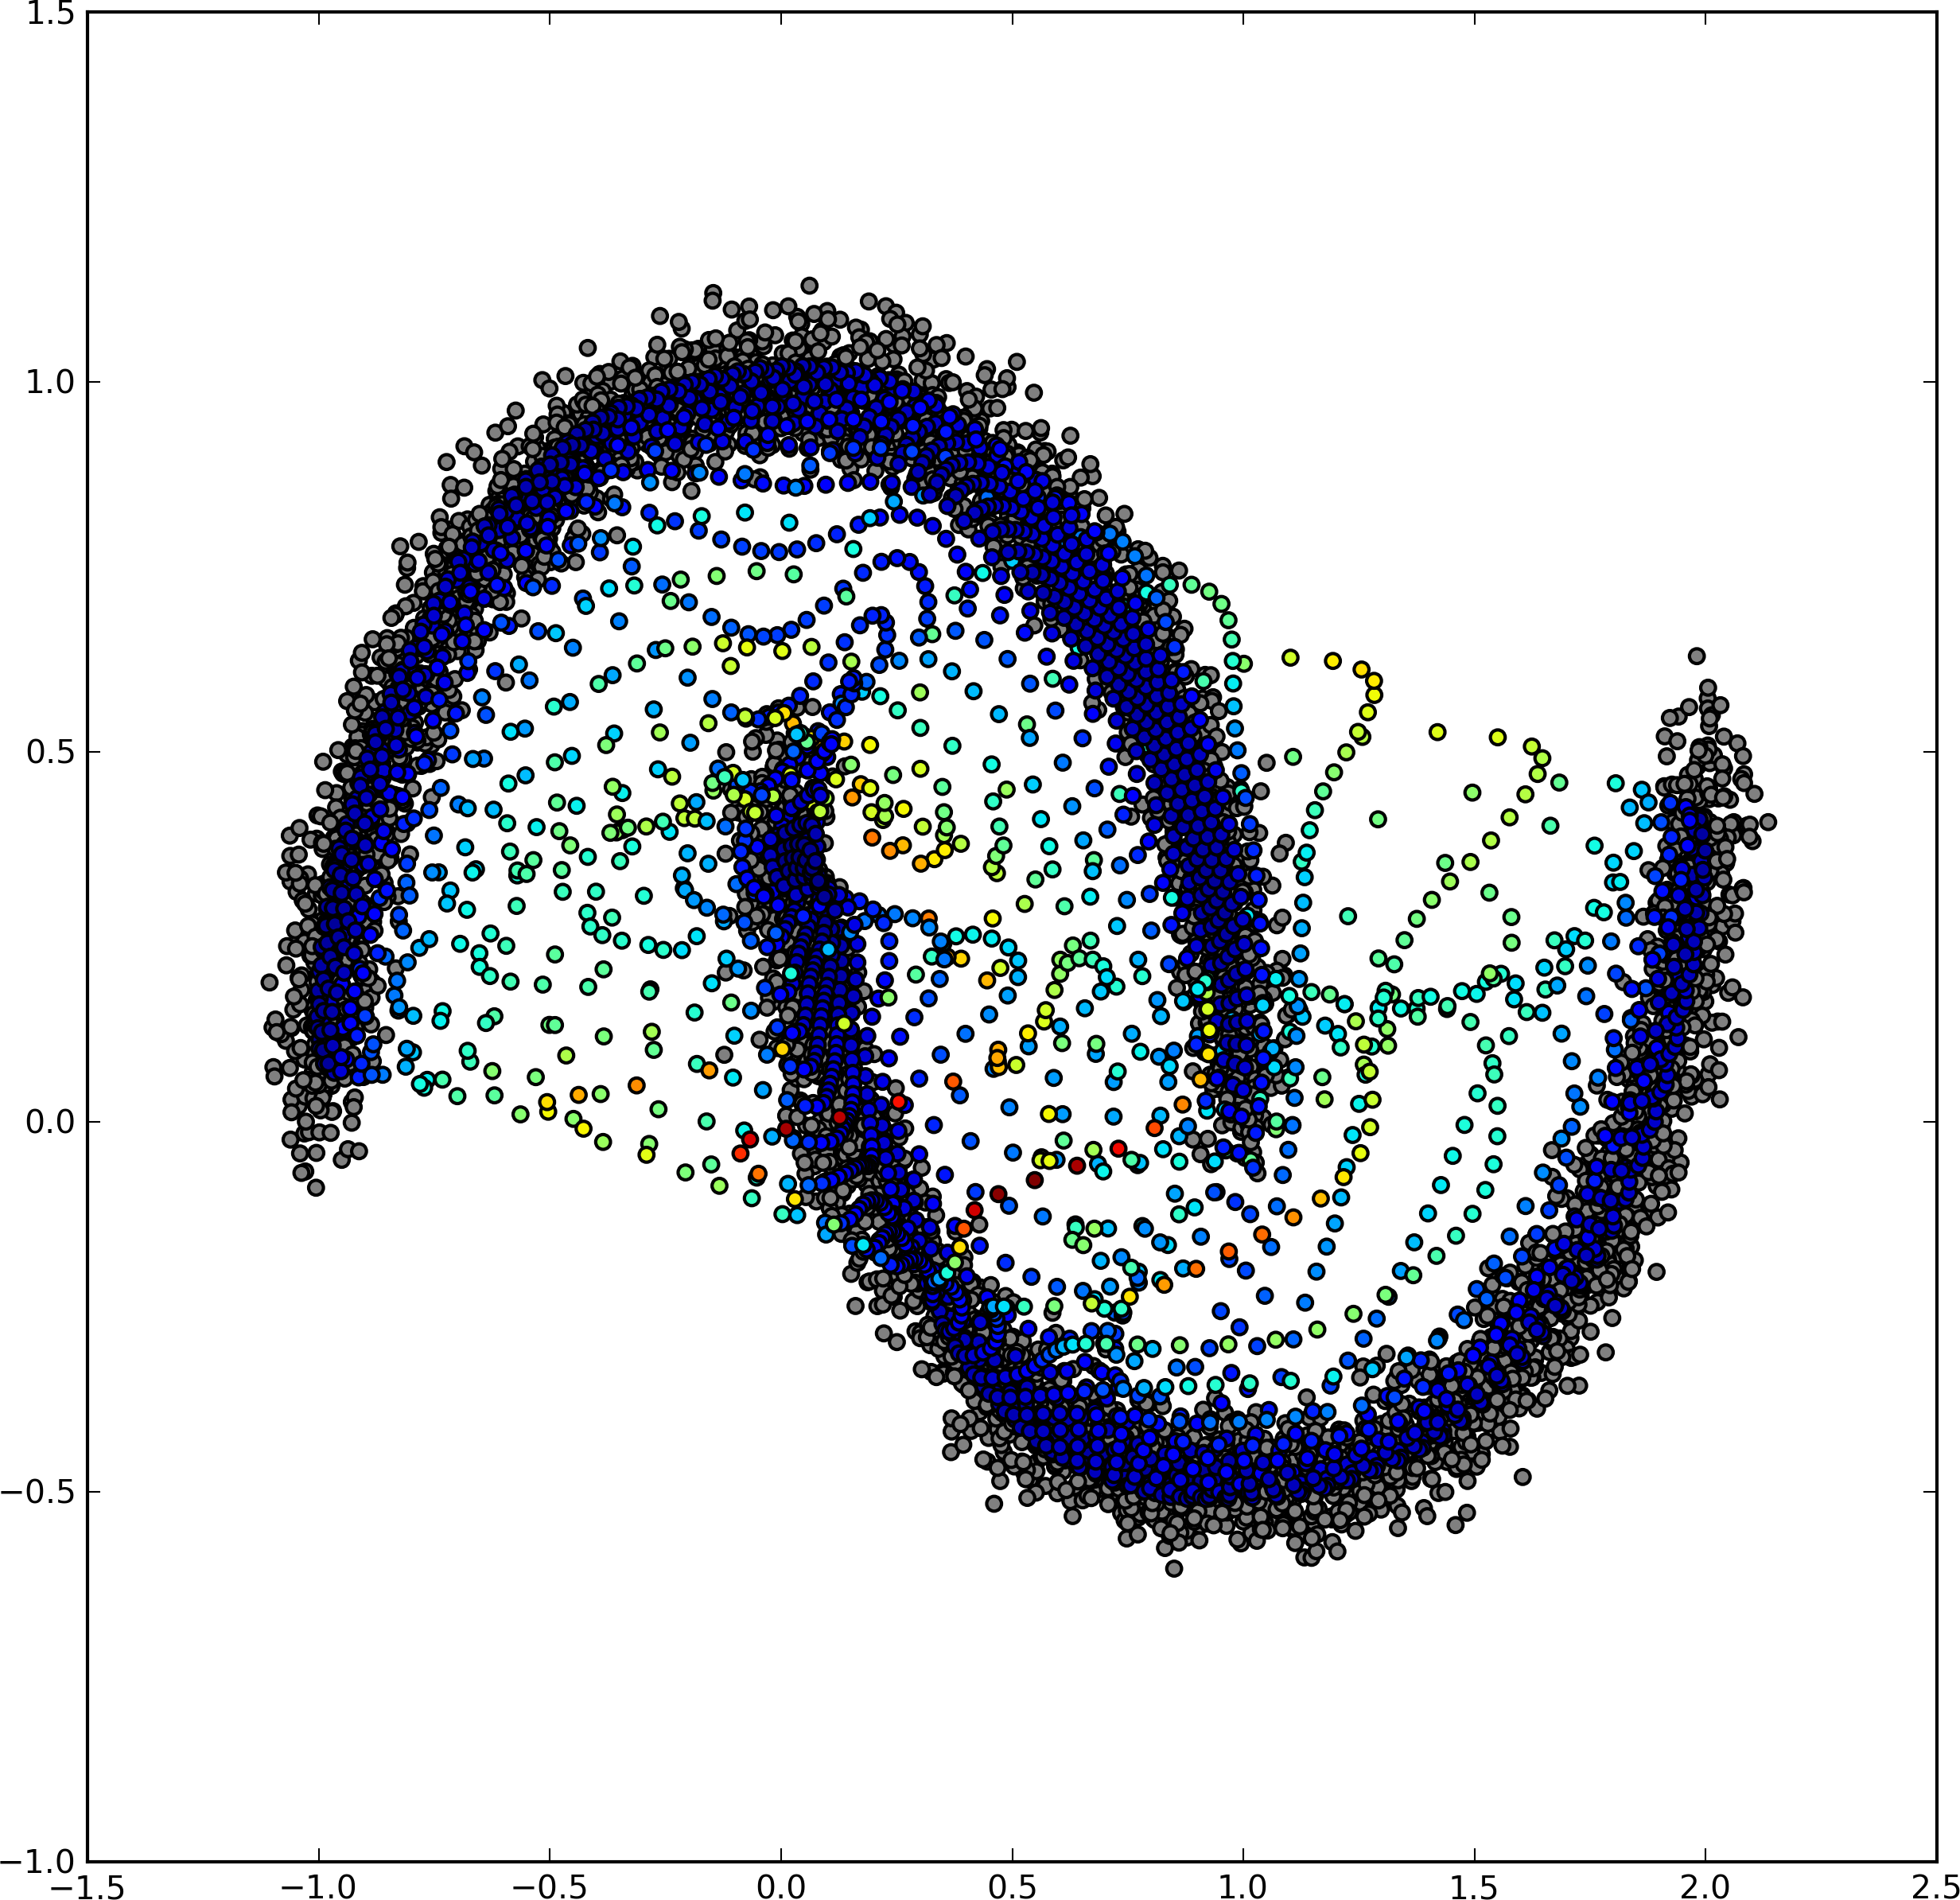
\includegraphics[width=\textwidth]{figures/somtrained_umat.png}
        \end{column}
    \end{columns}
    The U-matrix is a very conveniant tool to display the topology of the SOM. However the periodicity is not easily readable on the map.
}

\frame{
    \frametitle{Dealing with the donut!}
    \begin{columns}
        \begin{column}{0.6\textwidth}
            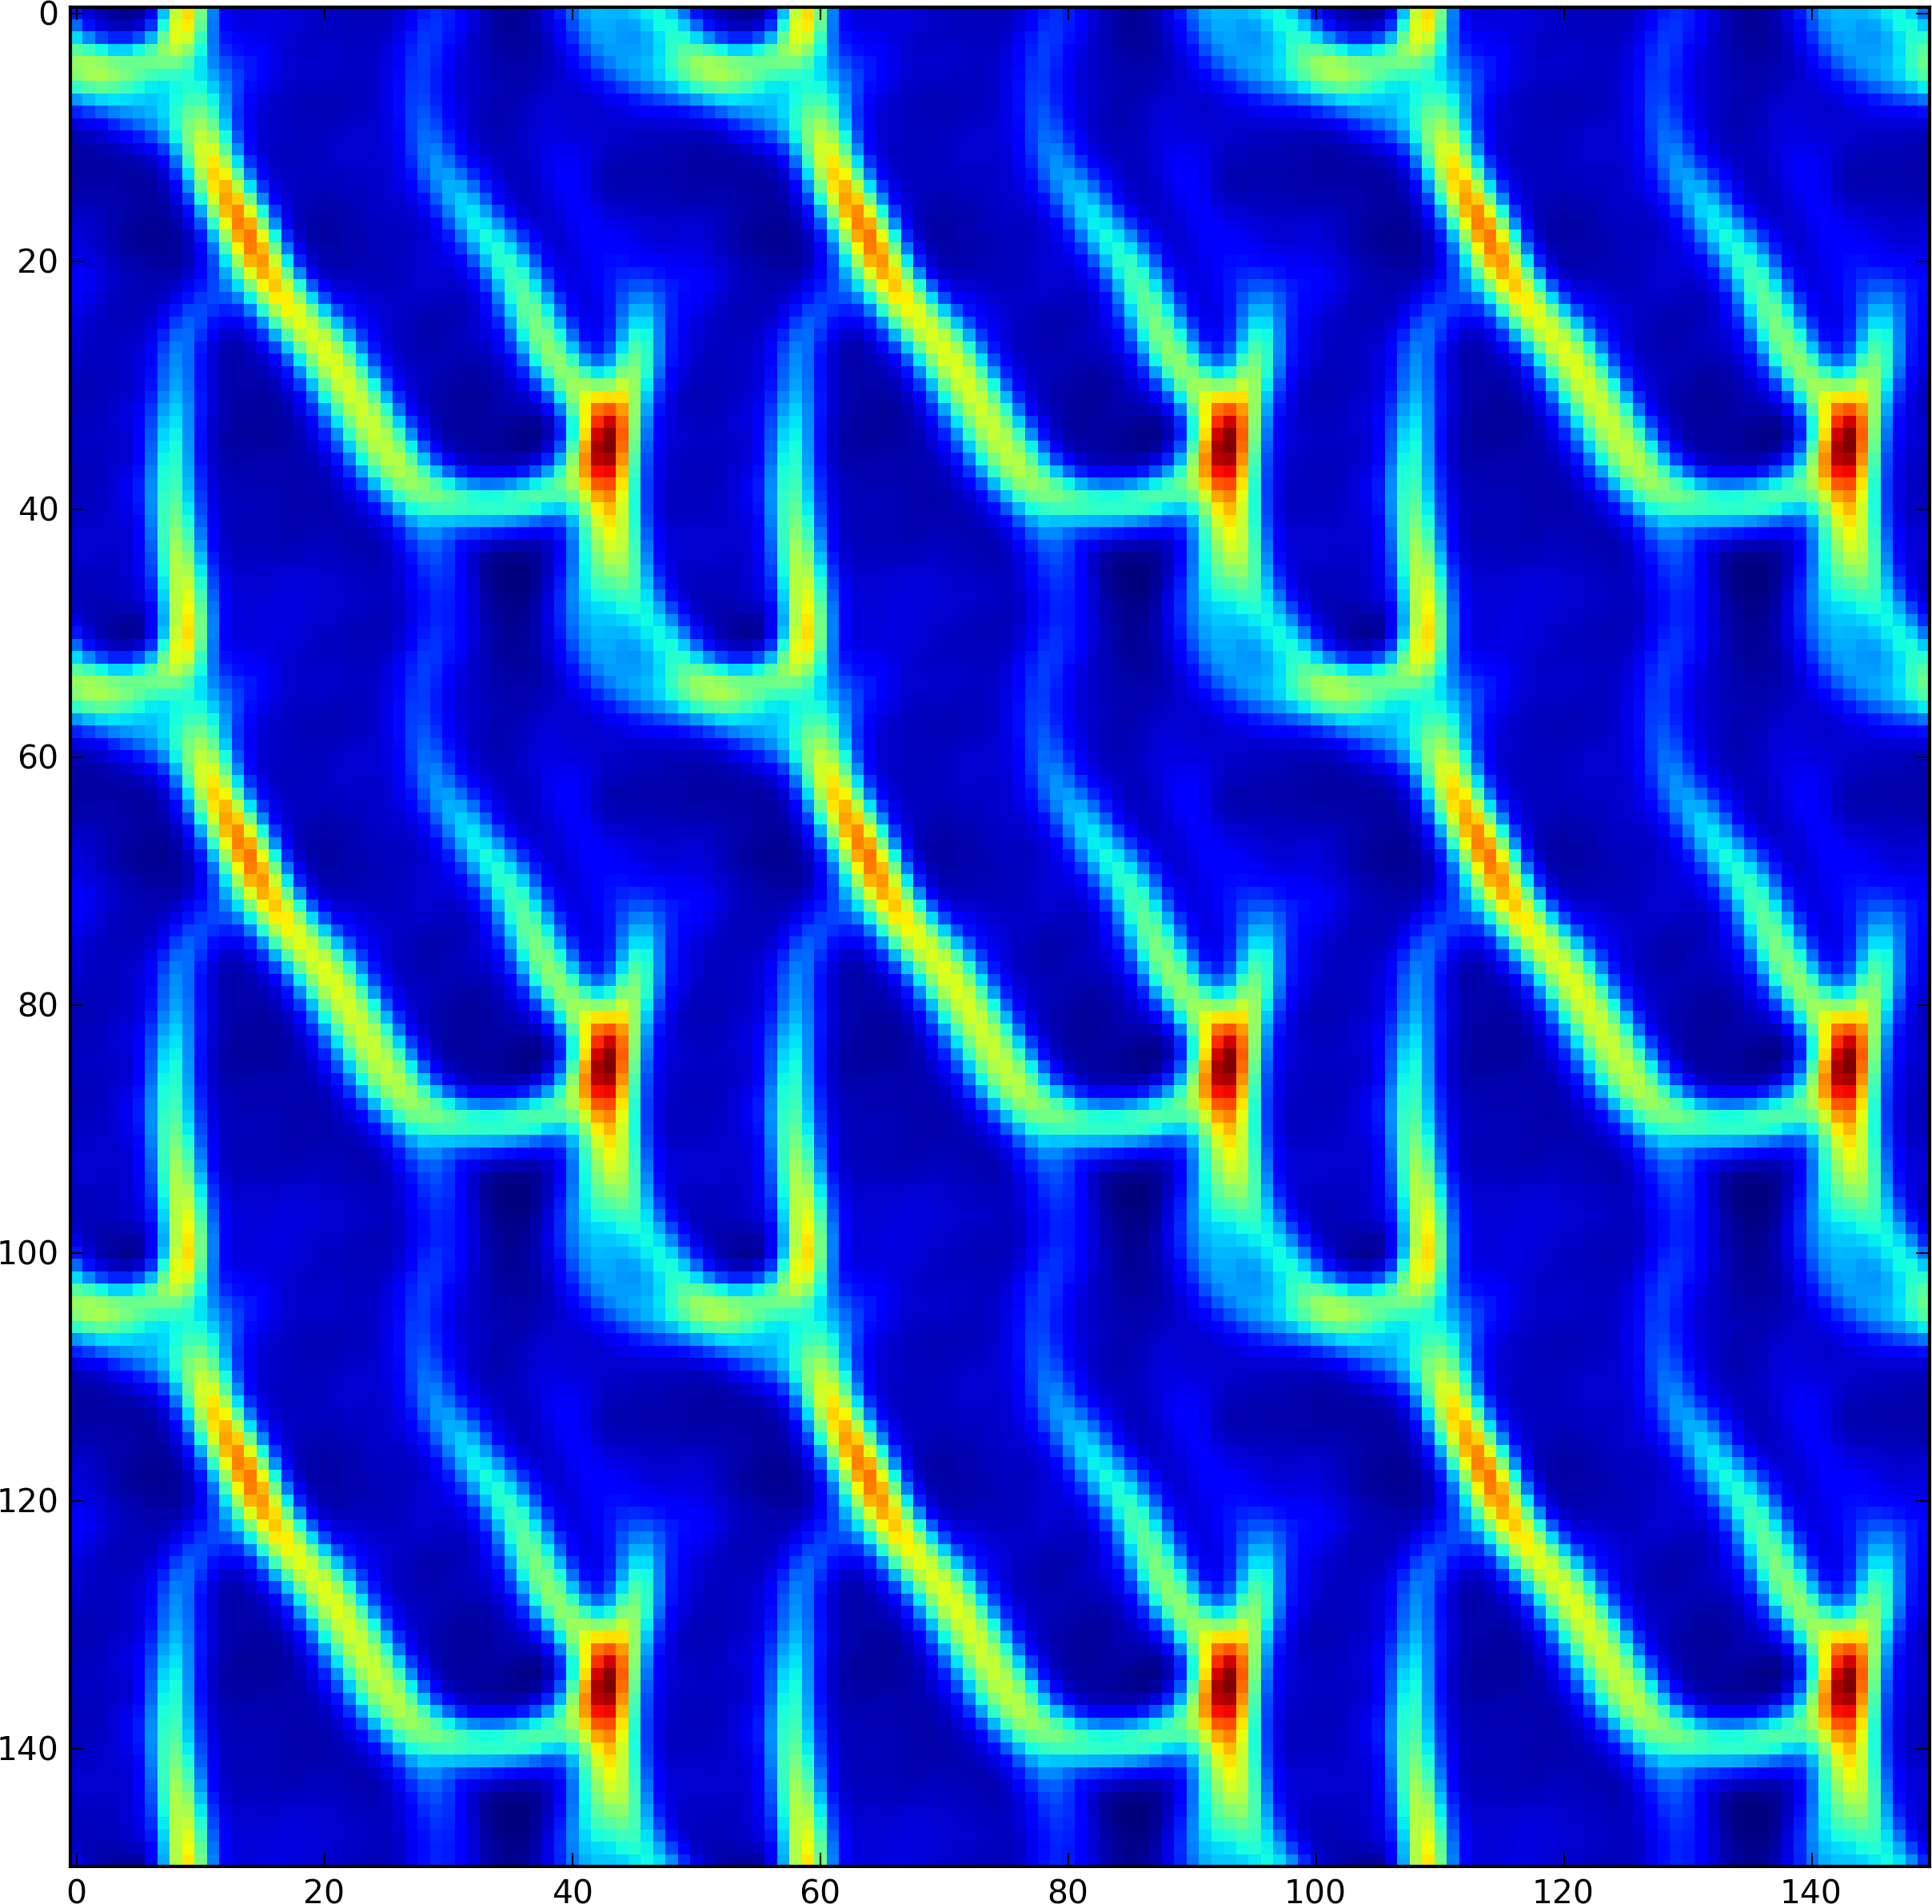
\includegraphics[width=\textwidth]{figures/umat_expand.png}
        \end{column}
        \begin{column}{0.4\textwidth}
            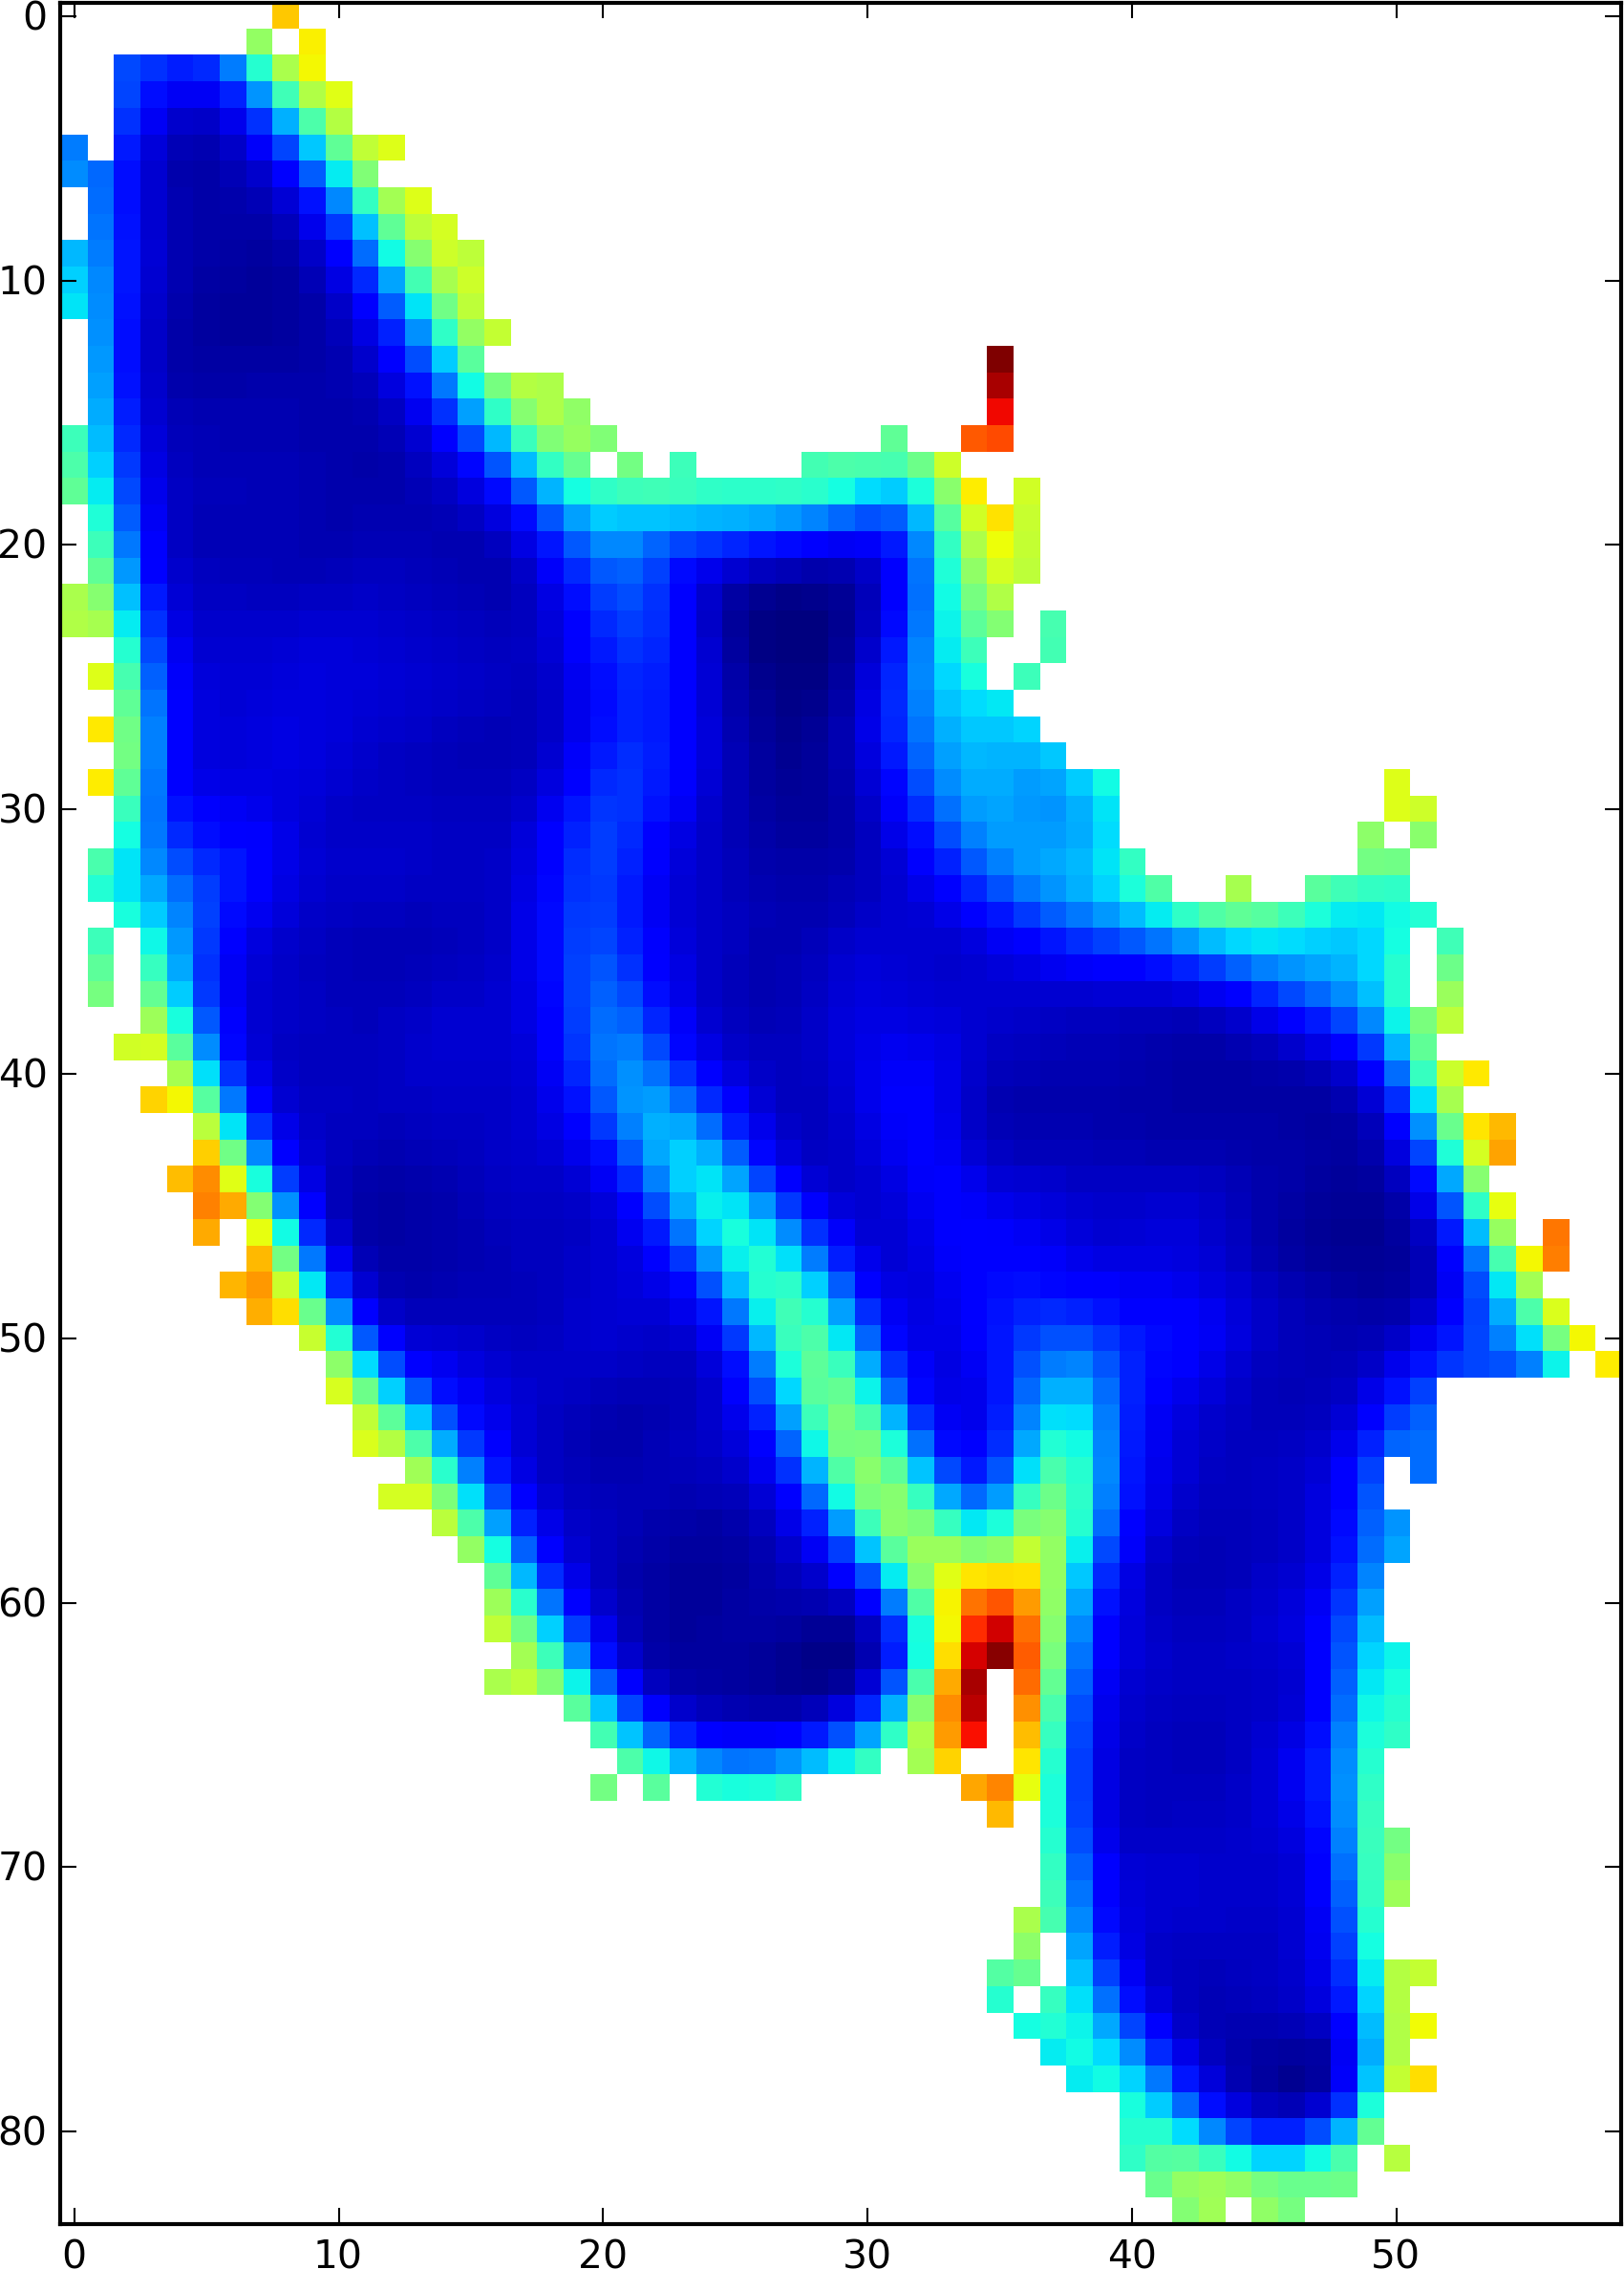
\includegraphics[width=\textwidth]{figures/umat_cont.png}
        \end{column}
    \end{columns}
    The algorithm -- called ``flooding algorithm'' -- starts from the global minimum of the U-matrix (many thanks to Mathias Ferber for this idea).
    It floods the map according to the relief of the U-matrix.
    This algorithm is inspired from the watershed algorithm.
}

\begin{frame}
    \frametitle{Clustering the U-matrix}
    The main advantage of the flooding algorithm is to define cluster according to the flooding process.
    Each time the level goes down a new cluster is define.
    From this point of view we can define ``natural cluster'' without dealing with threshold definition!
    \begin{columns}
        \begin{column}{.4\textwidth}
            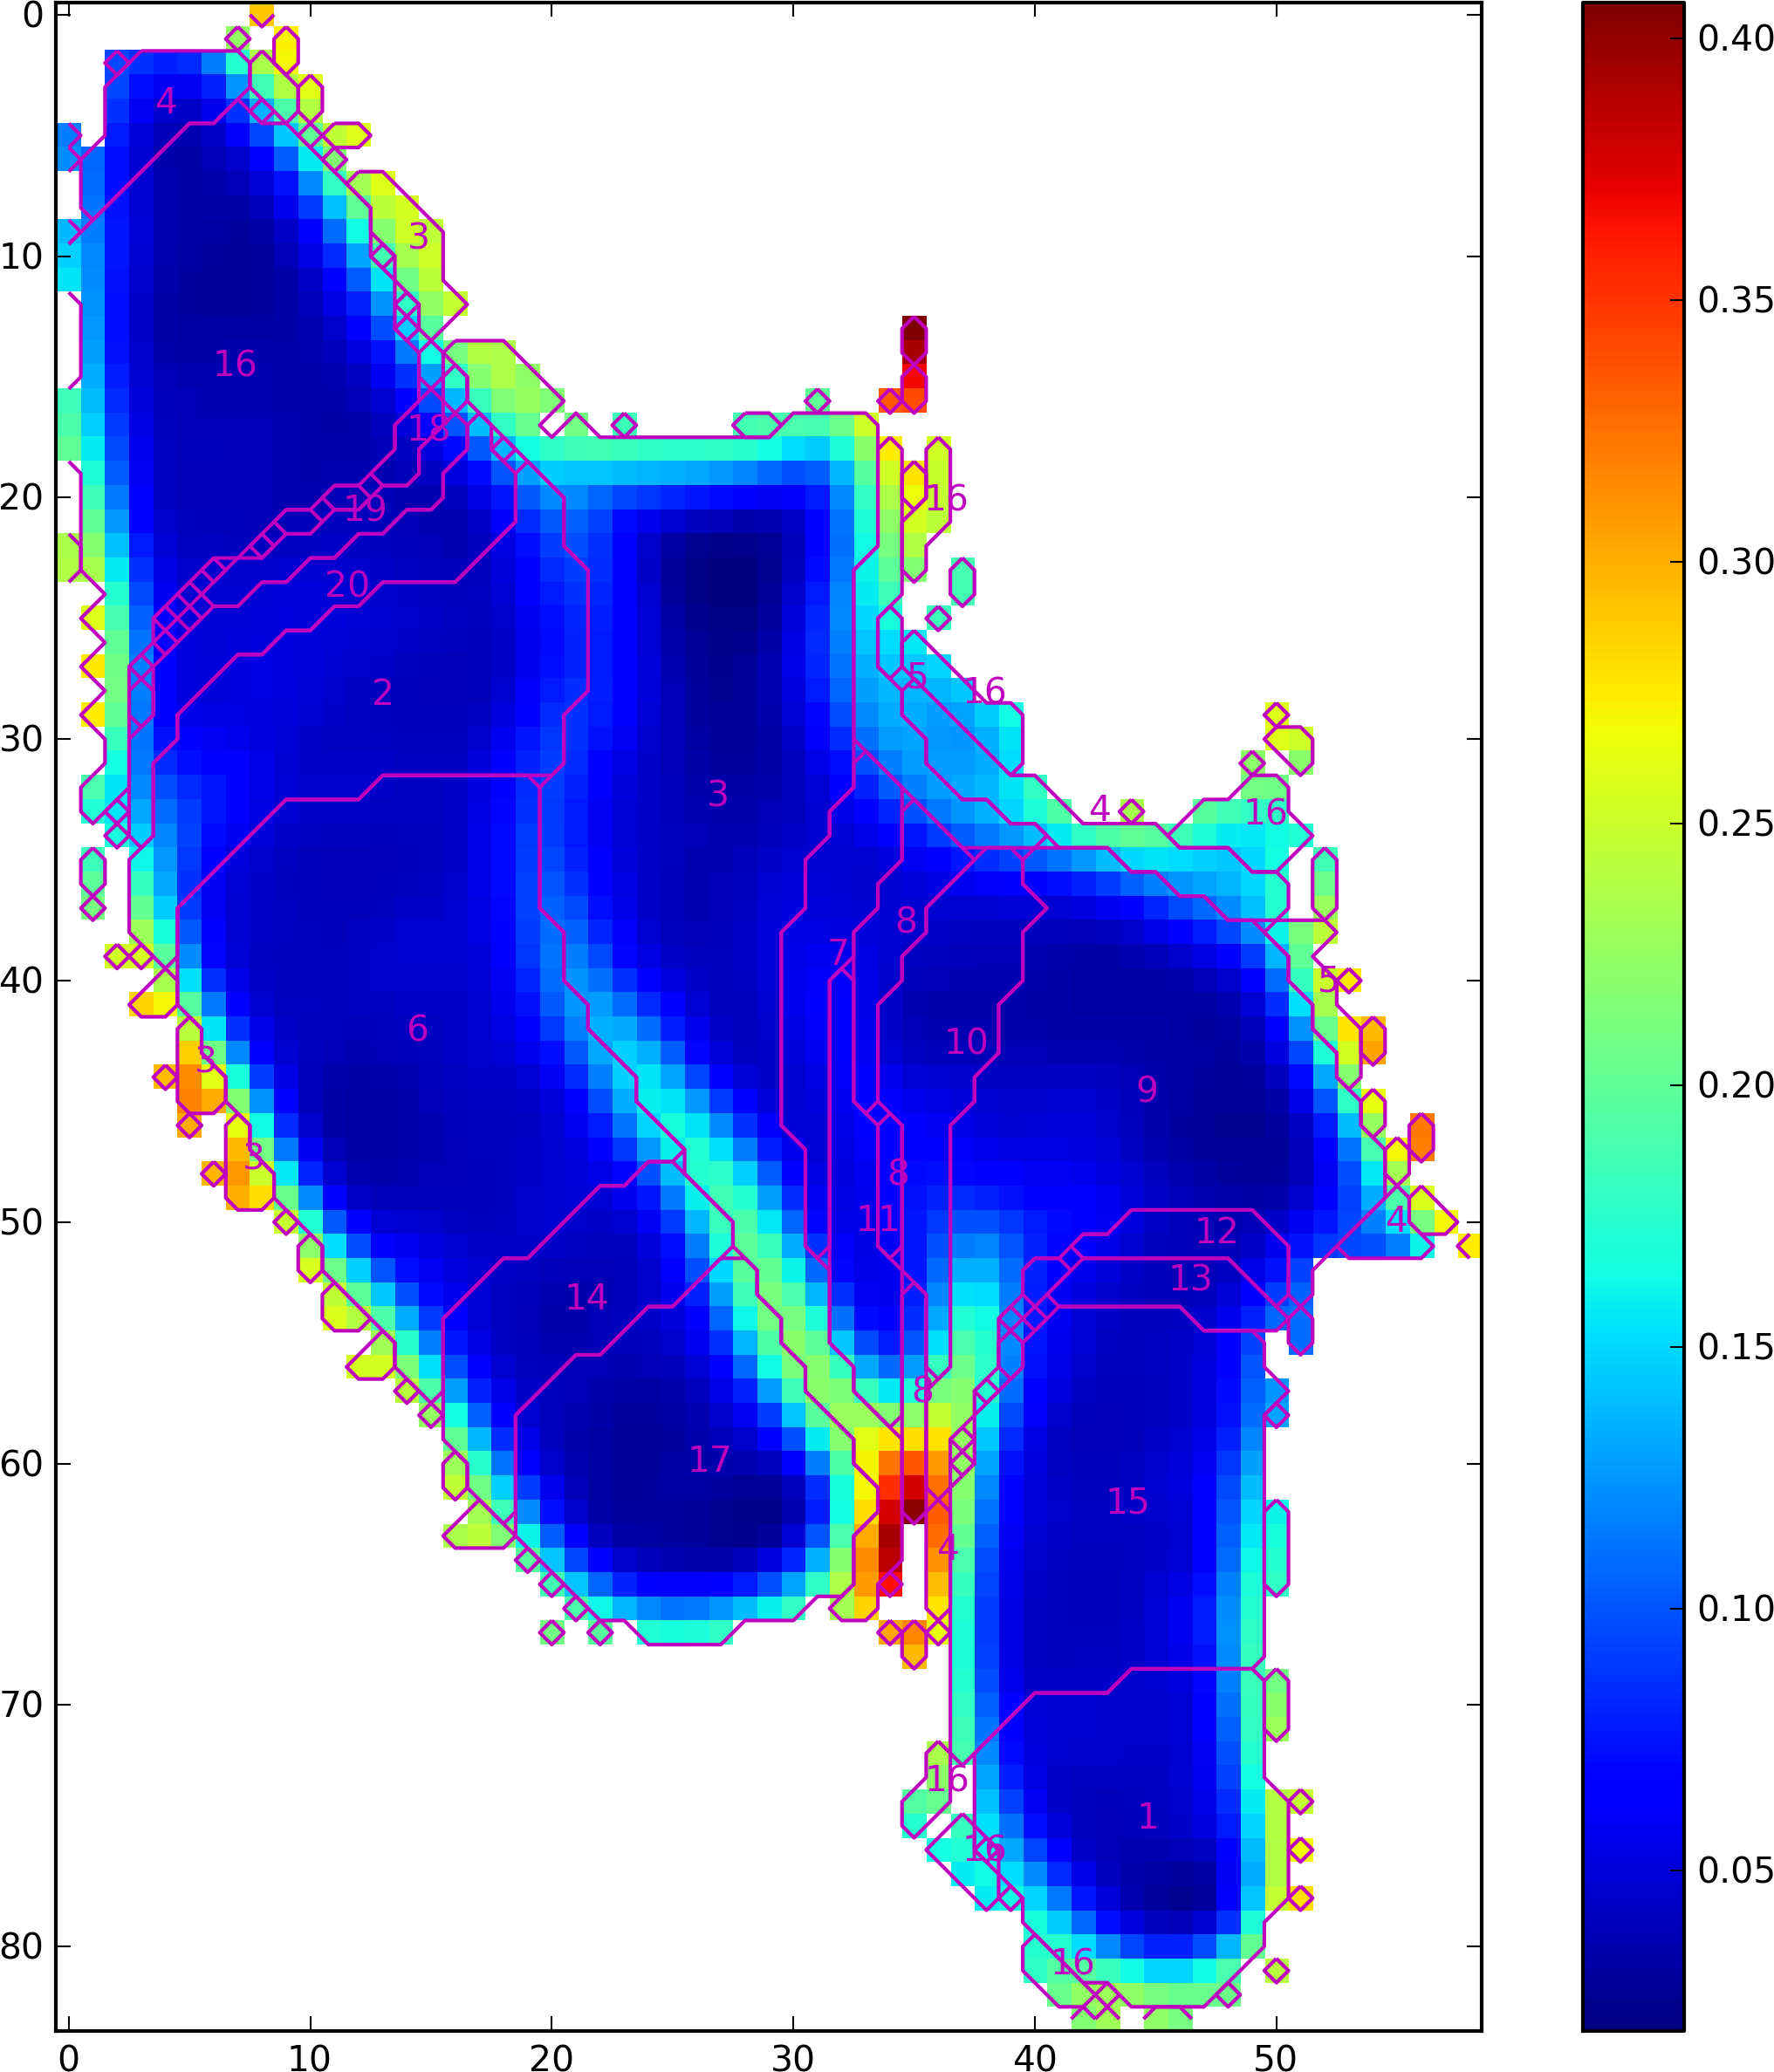
\includegraphics[width=\textwidth]{figures/umat_clust.png}
        \end{column}
        \begin{column}{.6\textwidth}
            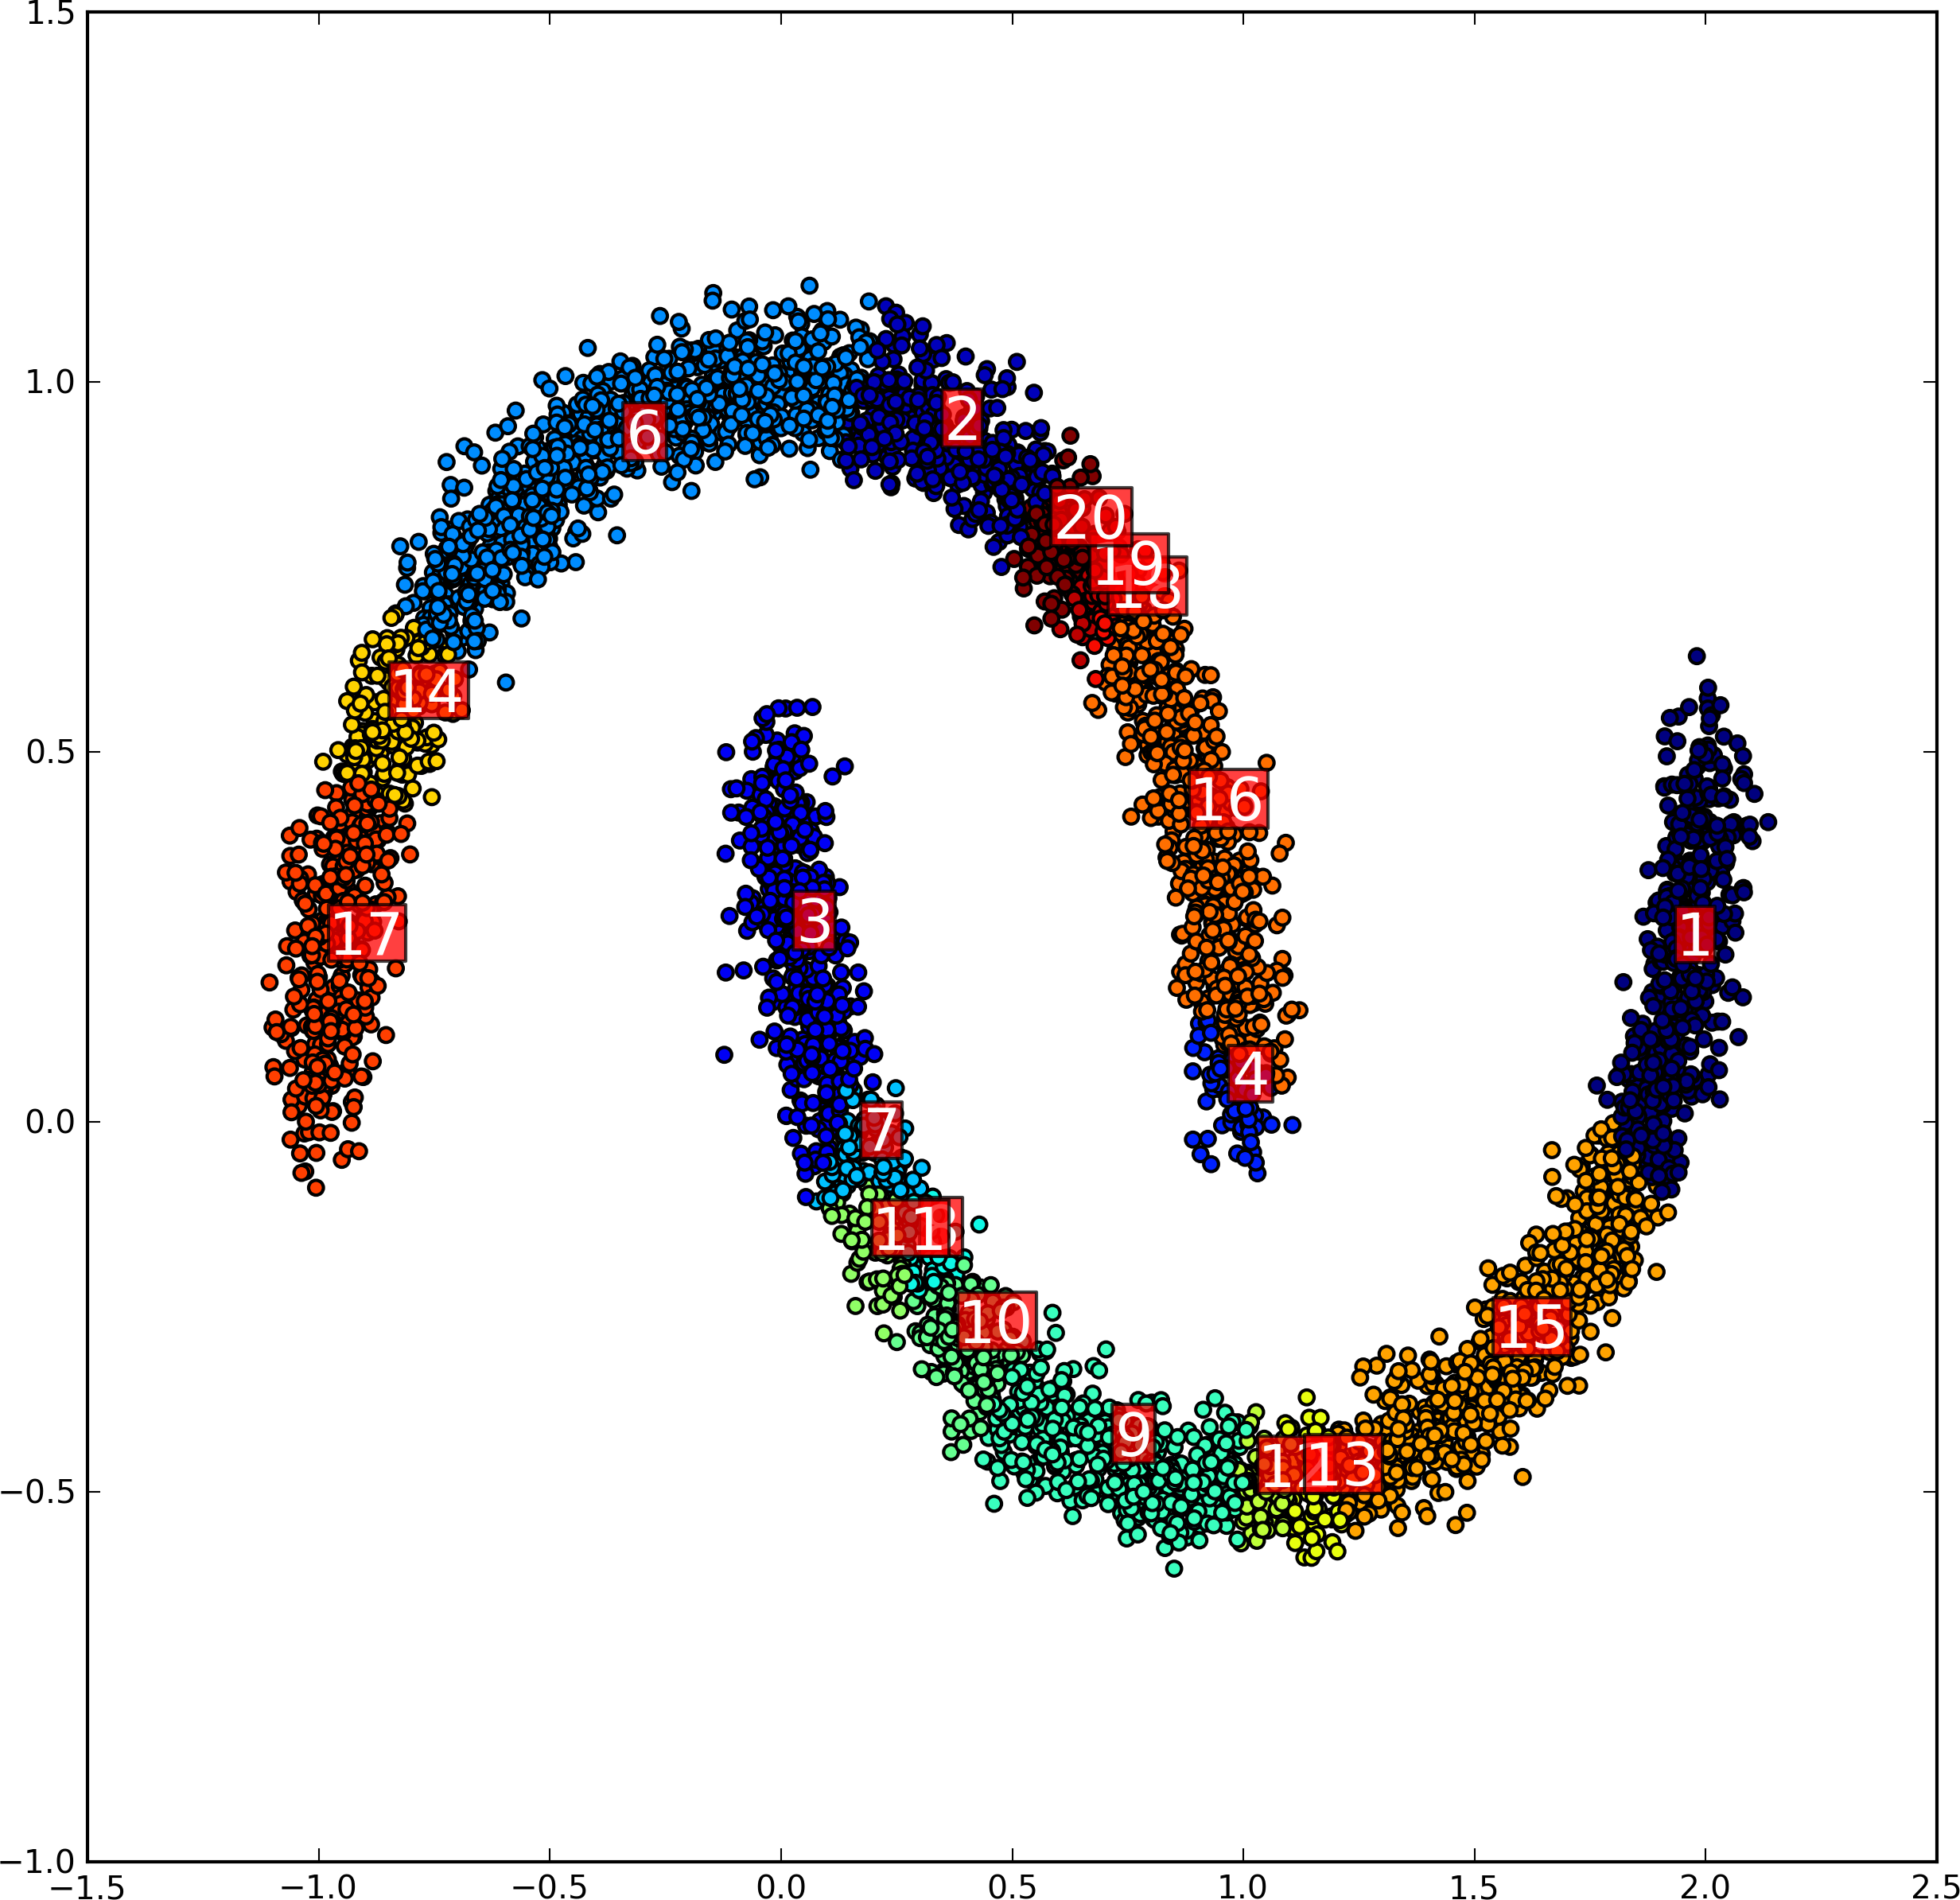
\includegraphics[width=\textwidth]{figures/moon_clust.png}
        \end{column}
    \end{columns}
\end{frame}

\section{Application to protein conformation clustering}
\frame{
\frametitle{How to describe a protein conformation?}
\begin{block}{Euclidean distance matrix}
$A=(a_{ij})$;
$a_{ij}=\|x_{i}-x_{j}\|_{2}^{2}$
where $\|x_{i}-x_{j}\|_{2}$ is the euclidean distance between the two atoms $x_{i},x_{j}$
\end{block}

\begin{block}{Spectral decomposition of distance matrix}

Decomposition based on eigenvalues of a square matrix $A$ is called spectral
decomposition. It allows us to express the original square matrix $A$ of size
$N$ in $N\times N$ terms of its eigenvalues $\lambda_k$ and corresponding
eigenvectors $v_k$\footnote{J Struct Funct Genomics. 2009 March; 10(1): 67--81.}

$$A=\sum_{k}\lambda_kv_kv_k^T$$
\end{block}
}

\frame{
\frametitle{How many PCs to describe a distance matrix?}
\begin{columns}
\begin{column}{.33\textwidth}
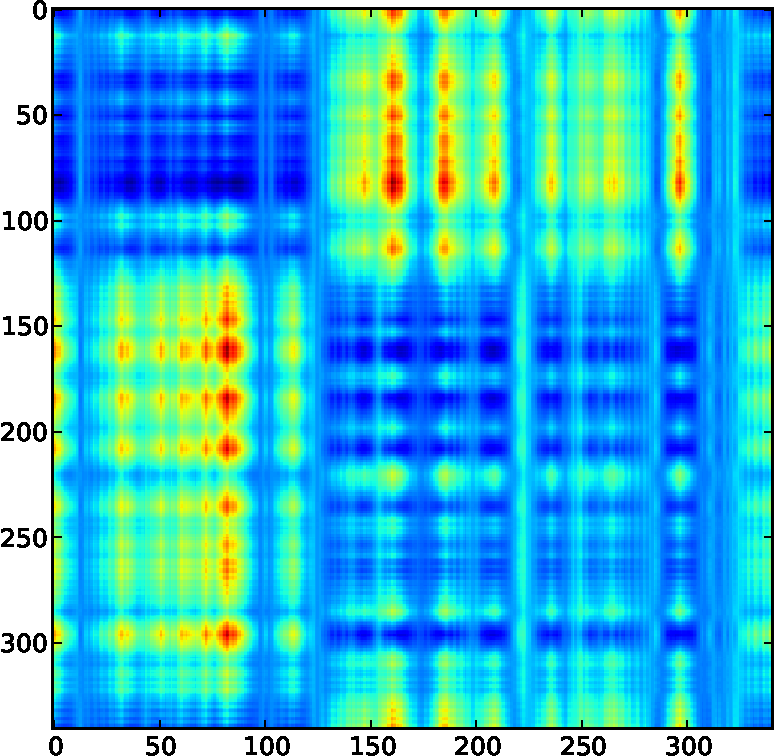
\includegraphics[width=\textwidth]{figures/distance_matrix_1PC-crop.pdf}\\
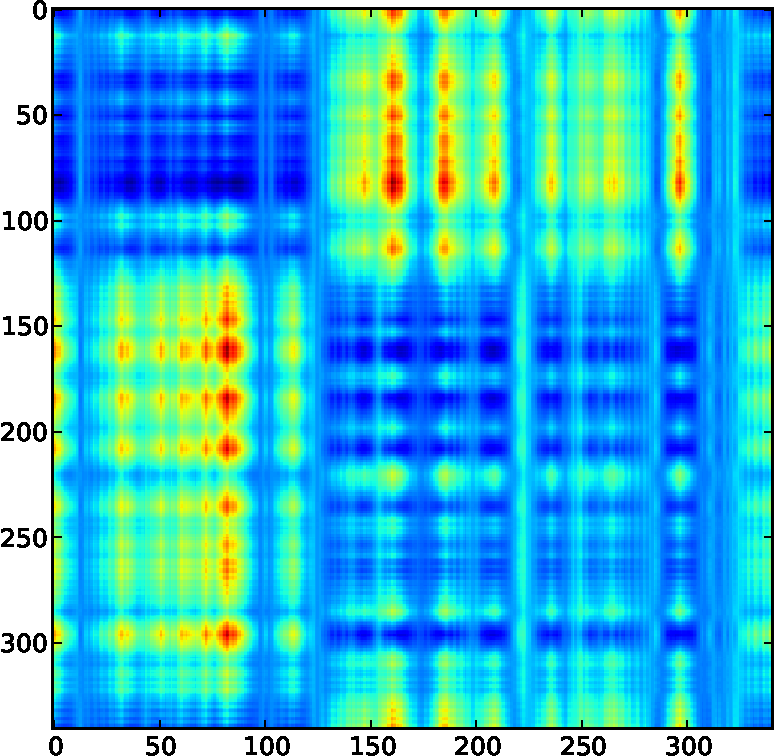
\includegraphics[width=\textwidth]{figures/distance_matrix_2PC-crop.pdf}
\end{column}
\begin{column}{.33\textwidth}
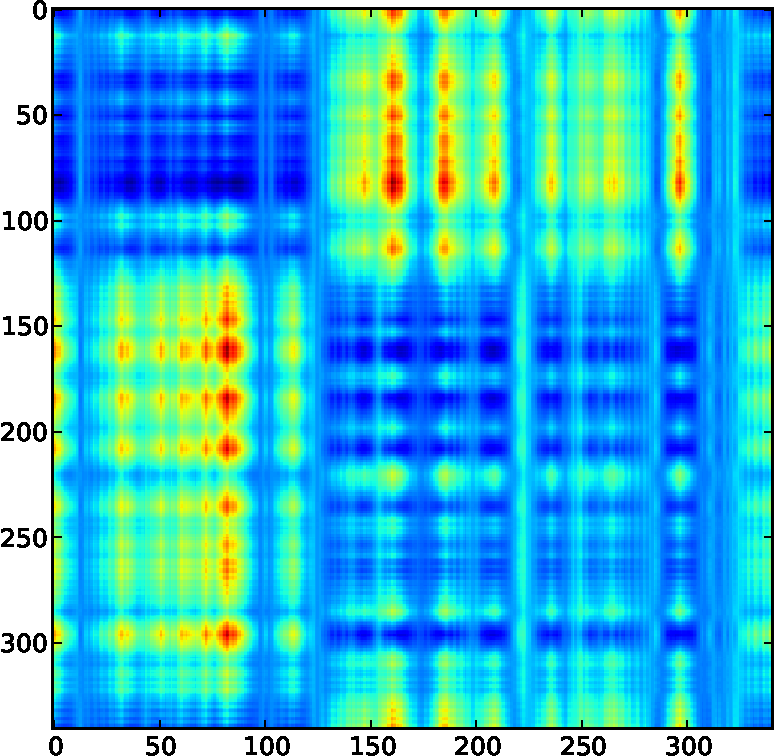
\includegraphics[width=\textwidth]{figures/distance_matrix_3PC-crop.pdf}\\
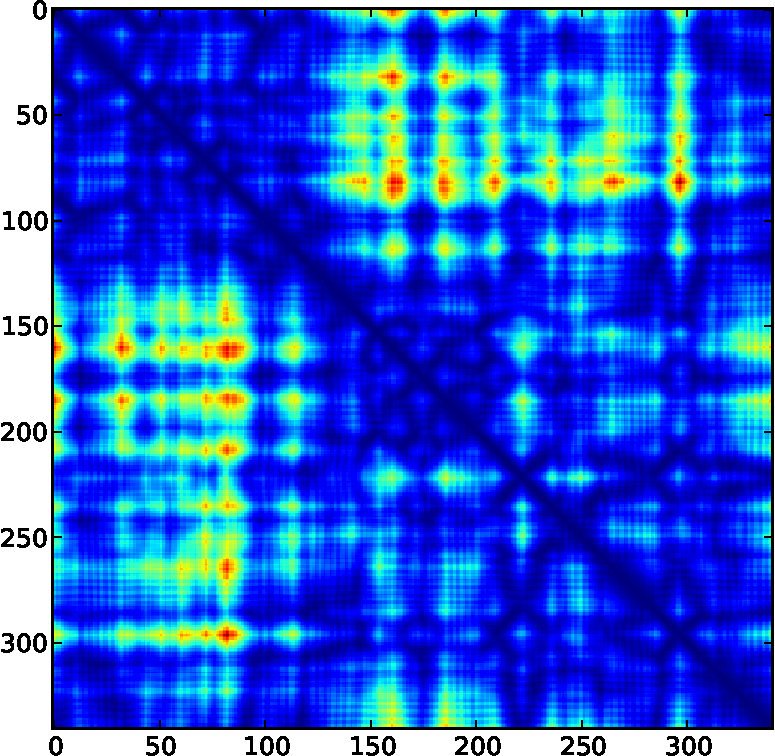
\includegraphics[width=\textwidth]{figures/distance_matrix_4PC-crop.pdf}
\end{column}
\begin{column}{.33\textwidth}
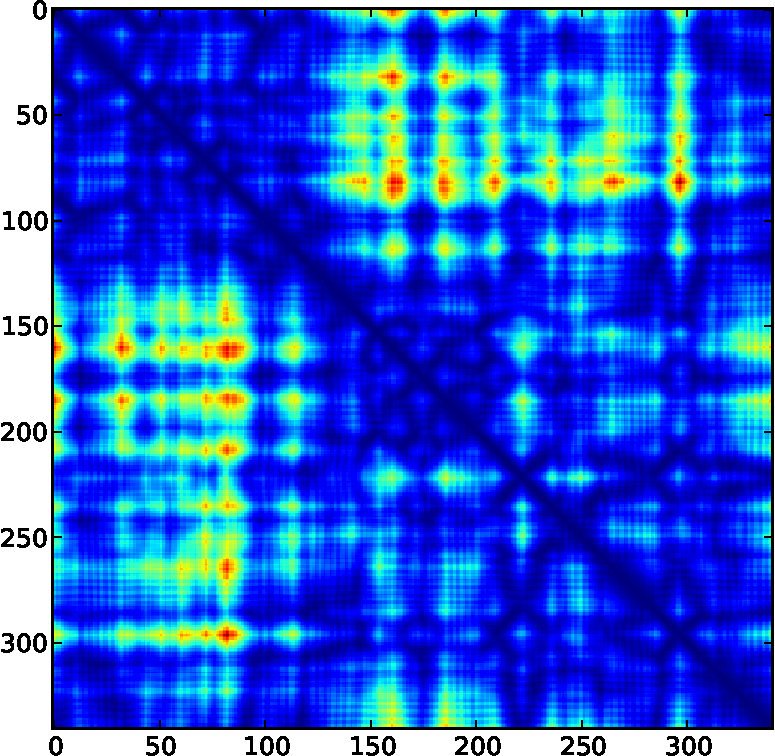
\includegraphics[width=\textwidth]{figures/distance_matrix-crop.pdf}\\
Matrix reconstruction of the original matrix above with 1, 2, 3 and 4 PCS.
\end{column}
\end{columns}
}

\frame{
\frametitle{Protein conformation descriptor}

\begin{alertblock}{The distance matrix}
The square distance matrix is too big to be an efficient descriptor: for a
protein with 341 amino-acids (VanA), a $C_\alpha$ distance matrix gives a
descriptor length of 57\,970. With 25\,000 snapshot the size of the input
matrix is: $25\,000 \times 57\,970$
\end{alertblock}

\begin{block}{The first 4 PCs...}

\textbf{The first 4 PCs of the PCA are sufficient to describe the distance matrix}. We
obtain a descriptor with 1\,364 elements and an input matrix with $25\,000
\times 1\,364$. The compression rate is 43.

\end{block}

\begin{exampleblock}{Advantages}

The clustering is not dependant of the alignment of the trajectory.

\end{exampleblock}

}

\begin{frame}
    \frametitle{Resistance mechanism to vancomycin antibiotic}
    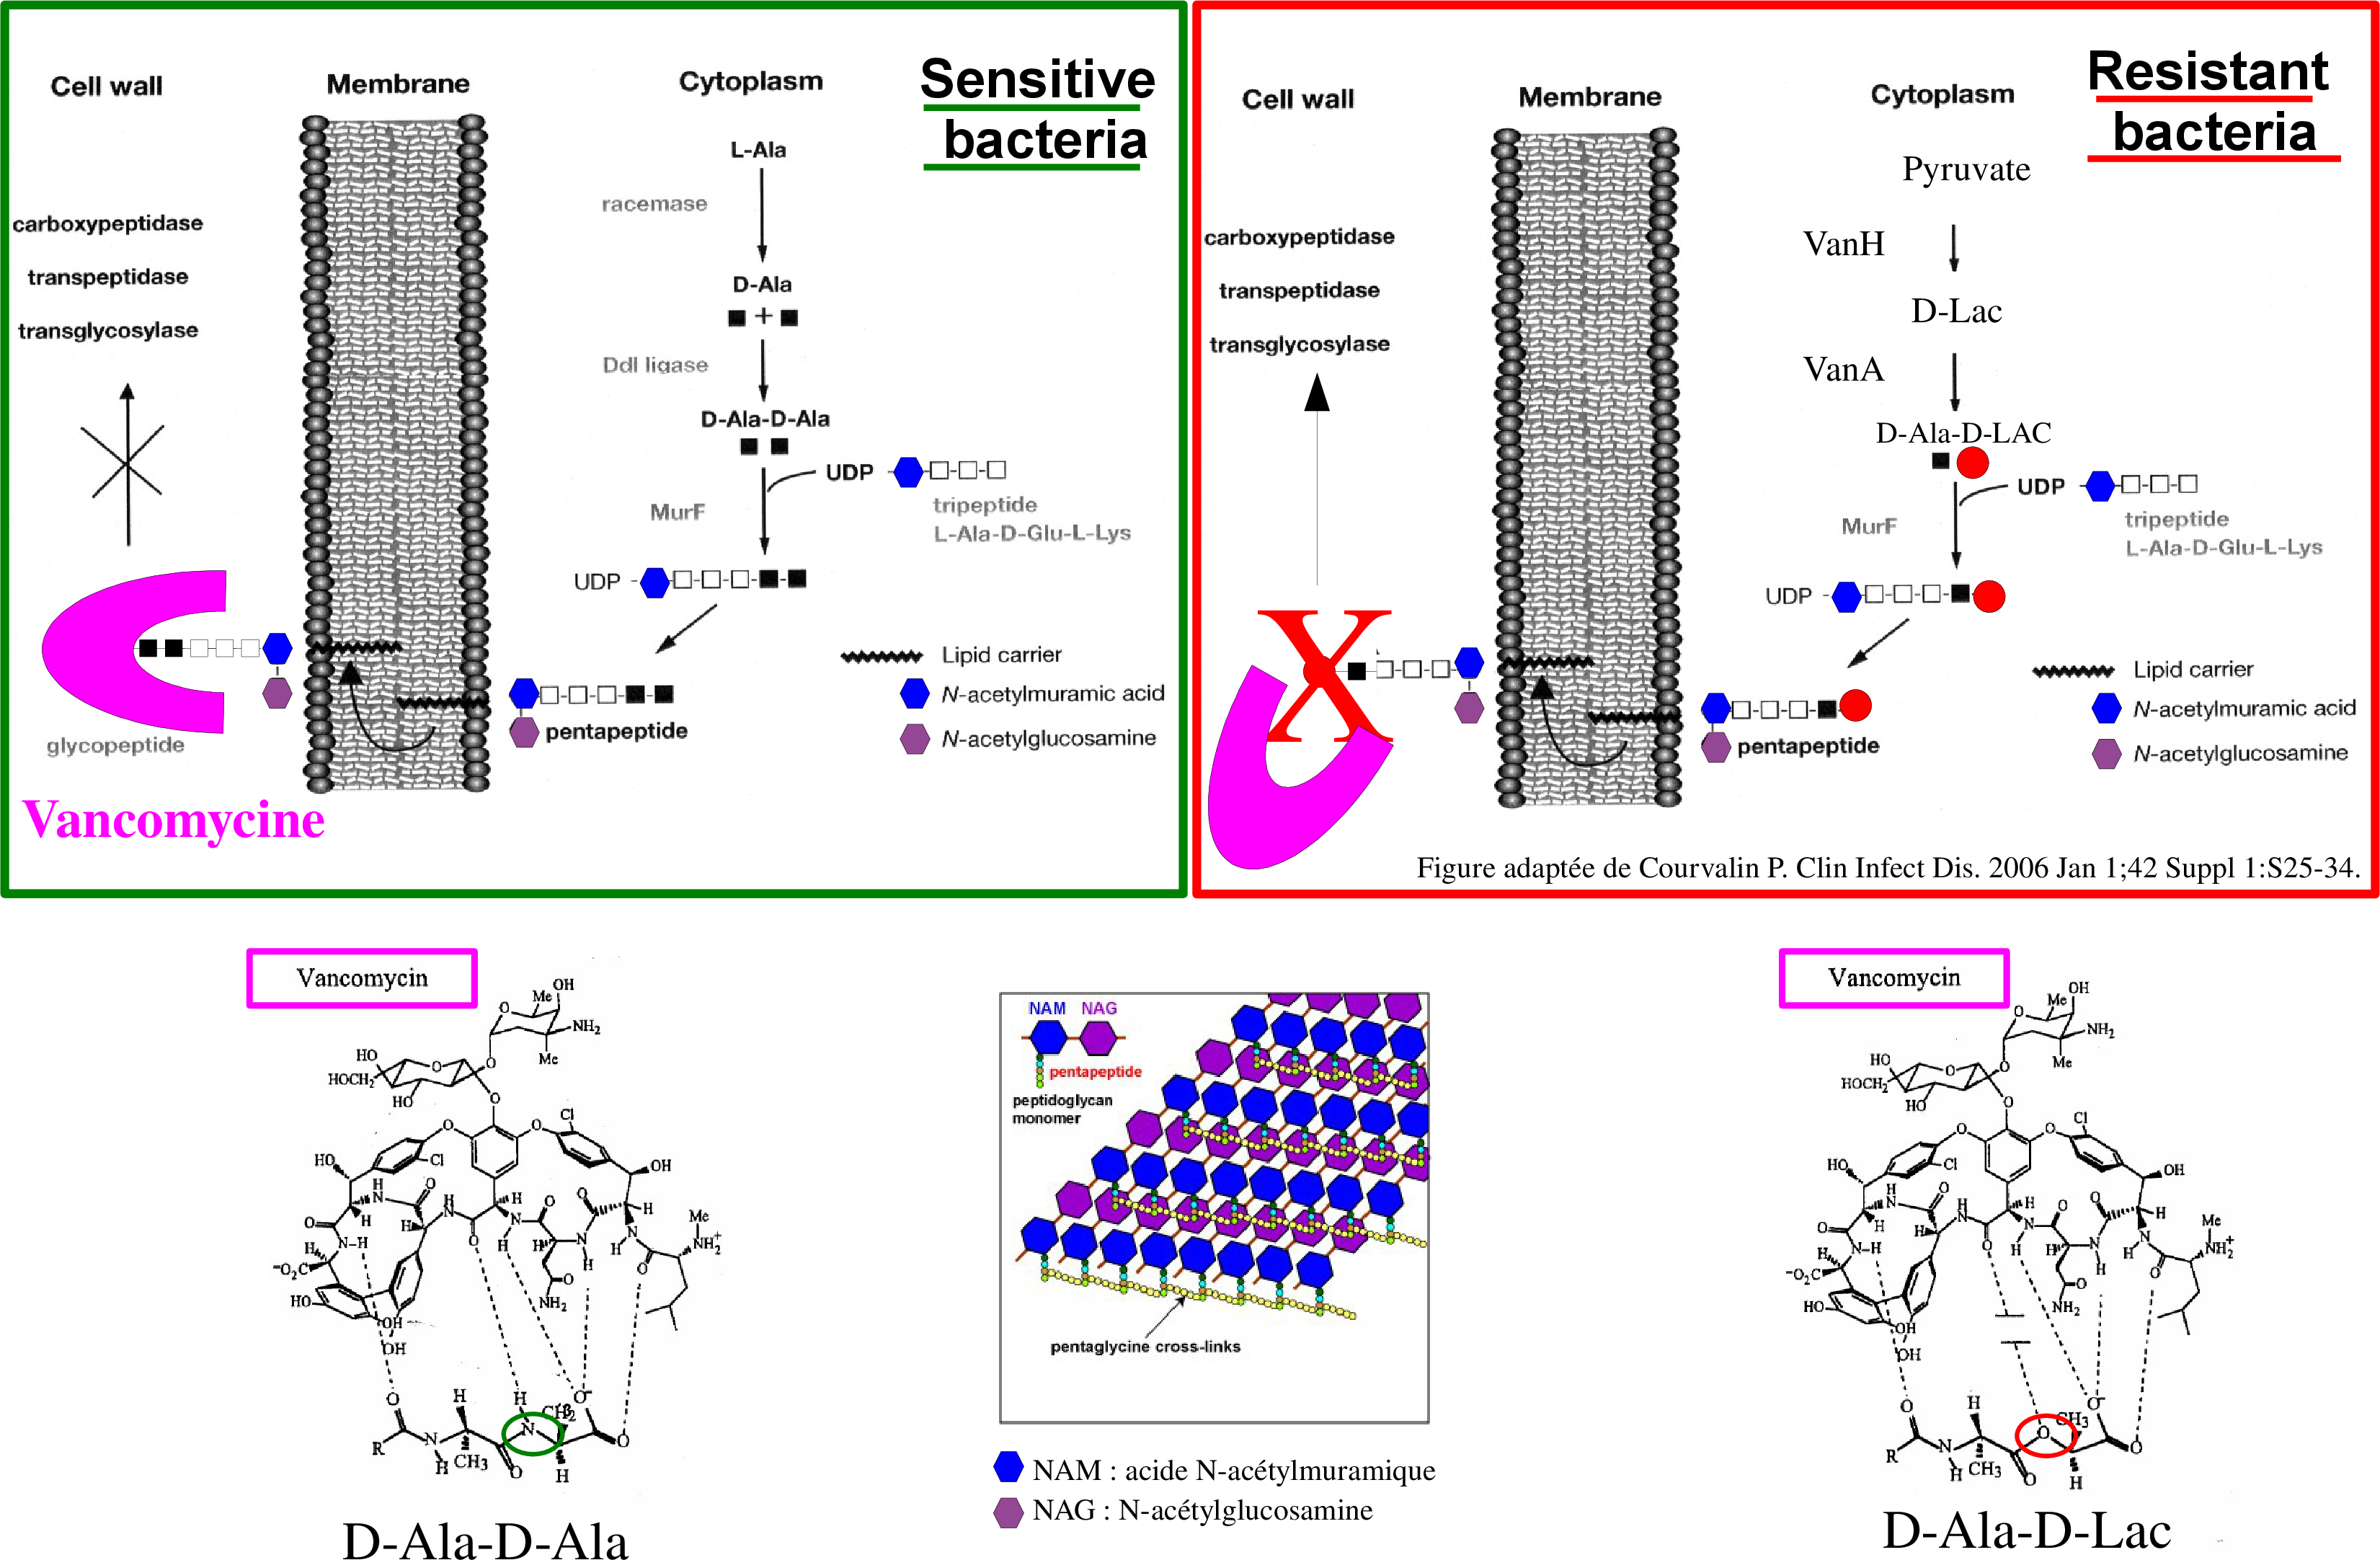
\includegraphics[width=\textwidth]{figures/ResistanceMechanism.png}
\end{frame}

\begin{frame}
    \frametitle{VanA molecular dynamics (25ns)}
    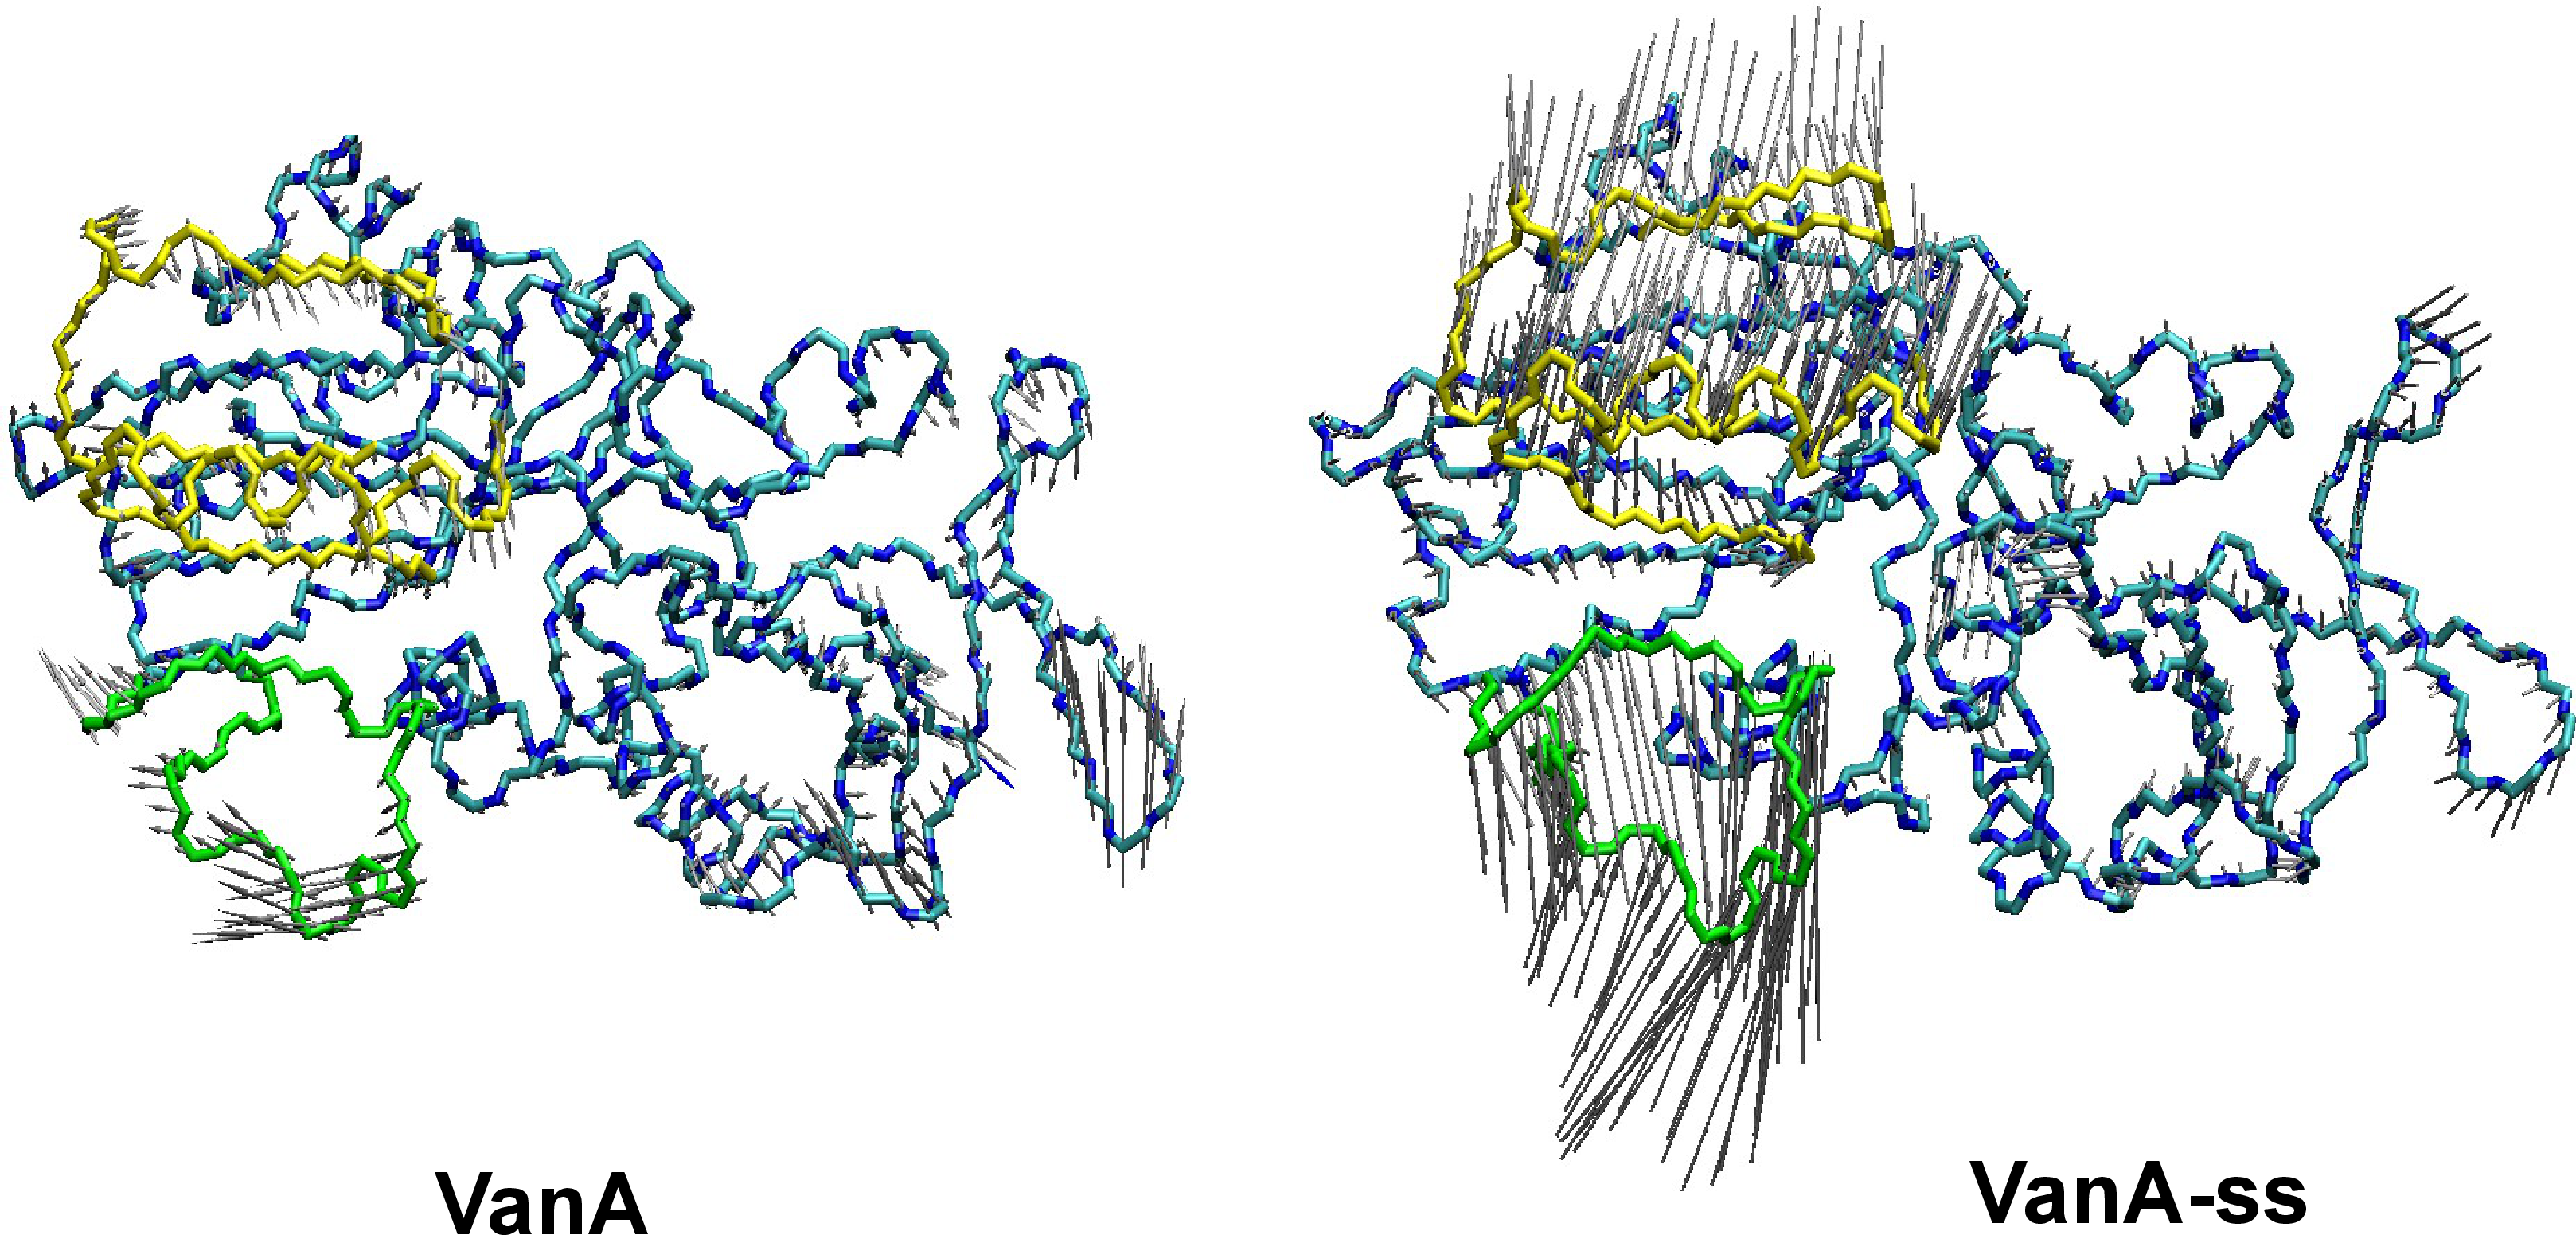
\includegraphics[width=\textwidth]{figures/PCA-2etats.png}

    PCA on VanA and VanA$_{ss}$.
\end{frame}

\section{How to do in practice?}
\begin{frame}
    \frametitle{Get the code}
    The code is on Github:
    
\includegraphics[width=.5\textwidth]{figures/github.png}\\
    \href{https://github.com/bougui505/SOM/tree/dev}{https://github.com/bougui505/SOM/tree/dev}\\
    And can be downloaded as a zip archive.

    It's written in \textbf{python} and need \textbf{numpy} and \textbf{scipy} libraries.

    Let's take a look on the code on Github.
\end{frame}

\end{document}

